\documentclass[12pt]{article}
\usepackage[a4paper, margin=1in, bindingoffset=1.5cm]{geometry}
\usepackage{graphicx}
\graphicspath{{images/}}
\usepackage{amsmath}
\usepackage{multirow}
\usepackage{multicol}
\usepackage{tgpagella}
\usepackage{url}
\usepackage{titlesec}
\usepackage{enumerate}
%\usepackage{gensymb}
\usepackage{float}
\usepackage[T1]{fontenc}
\usepackage{mathabx,graphicx}
\usepackage[ruled,longend,linesnumbered]{algorithm2e}
\usepackage{chngcntr}
\counterwithin{figure}{section}
\counterwithin{table}{section}
\counterwithin{equation}{section}
\def\Circlearrowleft{\ensuremath{%
		\rotatebox[origin=c]{180}{$\circlearrowleft$}}}
\def\Circlearrowright{\ensuremath{%
		\rotatebox[origin=c]{180}{$\circlearrowright$}}}
%\usepackage{mathabx}
\titleformat{\section}[display]
  {\normalfont\bfseries\scshape\LARGE}{Chapter \thesection}{0.3em}{}
\usepackage{setspace}

\usepackage{listings}
\usepackage{color} %red, green, blue, yellow, cyan, magenta, black, white
\definecolor{mygreen}{RGB}{28,172,0} % color values Red, Green, Blue
\definecolor{mylilas}{RGB}{170,55,241}
\definecolor{gray}{rgb}{0.5,0.5,0.5}
\definecolor{codegreen}{rgb}{0,0.6,0}
\definecolor{aliceblue}{rgb}{0.94, 0.97, 1.0}
\definecolor{islamicgreen}{rgb}{0.0, 0.56, 0.0}
\definecolor{cobalt}{rgb}{0.0, 0.28, 0.67}
\definecolor{darkblue}{rgb}{0.0, 0.0, 0.55}
\lstset{language=Matlab,%
    %basicstyle=\color{red},
	backgroundcolor=\color{aliceblue},  
		basicstyle=\ttfamily,
		keywordstyle=\color{darkblue}\ttfamily,
		stringstyle=\color{mylilas}\ttfamily,
		commentstyle=\color{gray}\ttfamily,
		morecomment=[l][\color{codegreen}]{\#},
		breaklines=true,
		showstringspaces=false,
		tabsize=4,
		emph={%  
    for, end, break, while, if, else%
    },emphstyle={\color{darkblue}\bfseries}%%
}

\renewcommand{\baselinestretch}{1.5} 
\newcommand\tab[1][1cm]{\hspace*{#1}}

\begin{document}
\pagenumbering{gobble}
\begin{center}
%\vspace*{0.7cm}

\includegraphics[scale=0.70]{1}
\linebreak
\vspace*{-0.4cm}
\begin{LARGE}
\textbf{Adaptive Robust Local Complete Pattern For Facial Expression Recognition}\\
\end{LARGE}
\vspace*{0.9cm}
\textbf{Authors}\\
Al Shahriar Rubel (144434)\\
Adib Ahsan Chowdhury (144446)\\
\vspace*{0.9cm}
\textbf{Supervisor}\\
Dr. Md. Hasanul Kabir\\
Professor\\
Department of Computer Science and Engineering (CSE)\\
Islamic University of Technology (IUT)\\
\vspace*{1.2cm}
\textbf{A thesis submitted to the Department of CSE}\\
\textbf{in partial fulfillment of the requirements for the degree of\\B.Sc. Engineering in CSE}\\
\vspace*{0.7cm}
\textbf{October - 2018}
\end{center}
\newpage
\begin{center}
\begin{large}
\textbf{Declaration of Authorship}
\end{large}
\end{center}
\vspace*{.5cm}

\noindent This is to certify that the work presented in this thesis is the outcome of the analysis and experiments carried out by Al Shahriar Rubel and Adib Ahsan Chowdhury under the supervision of Dr. Md. Hasanul Kabir, Professor, Department of Computer Science and Engineering, Islamic University of Technology (IUT), Dhaka, Bangladesh. It is also declared that neither of this thesis nor any part of this thesis has been submitted anywhere else for any degree or diploma. Information derived from the published or unpublished work of others has been acknowledged in the text and a list of references is given.

\vspace*{1cm}
\noindent\textit{\Large{\textbf{Authors:}}}\\

\vspace*{1cm}
\noindent -----------------------------------------------------------------------\\
\noindent Al Shahriar Rubel\\
\noindent Student ID: 144434\\ 

\vspace*{1cm}
\noindent -----------------------------------------------------------------------\\
Adib Ahsan Chowdhury\\
Student ID: 144446\\

\vspace*{.7cm}
\noindent\textit{\Large{\textbf{Supervisor:}}}\\

\vspace*{.7cm}
\noindent -----------------------------------------------------------------------\\
Dr. Md. Hasanul Kabir\\
Professor,\\
Department of Computer Science and Engineering (CSE)\\
Islamic University of Technology (IUT)
\newpage
\addcontentsline{toc}{section}{Abstract}
\pagenumbering{roman}
\topskip0pt
\vspace*{2cm}
\begin{LARGE}
\begin{center}
\textbf{Abstract}
\end{center}
\end{LARGE}
\vspace*{0.7cm}

An effective and robust face descriptor is an essential component for a good facial expression recognition system. Many popular appearance-based methods such as local binary pattern (LBP), local directional pattern
(LDP) and local ternary pattern (LTP) have been proposed to serve this purpose and have been proven both accurate and
efficient. During the last few years, many researchers have been providing significant effort and ideas to improve these methods. In this research work, we present a new face descriptor, Adaptive Robust Local Complete Pattern (ARLCP). ARLCP  effectively encodes significant information of emotion-related features by using the sign, magnitude and directional information of edge response that is more robust to noise and illumination variation. In this histogram-based approach, obtained feature image is divided into several regions, histogram of each region is computed independently and all histograms are concatenated to generate a final feature vector. We have experimented our method on several datasets using cross-validation schemes to evaluate the performance. From those experiments, it is evident that our method(ARLCP) provides better accuracy in facial expression recognition.
\newpage
\addcontentsline{toc}{section}{Acknowledgement}
\topskip0pt
\begin{LARGE}
\begin{center}
\textbf{Acknowledgements}
\end{center}
\end{LARGE}
\vspace*{0.7cm}

First of all, we are really grateful the Almighty Allah for everything that happened in our life. Without His help, blessings and mercy, nothing would have been possible. ``All the thanks and praises to Allah''.\\
\linebreak
\noindent We would like to thank our supervisor,\textbf{ Dr. Md. Hasanul Kabir}, Professor, Department of Computer Science and Engineering, Islamic University of Techonology, Gazipur, Bangladesh for his kind advice, support and counsel. Dr. Kabir has been an instrumental to this
work and our careers. He taught us to work in research sectors and how to generate new ideas for solving problems. He also helped us to think out of the box to generate ideas like Adaptive Robust Local Complete Pattern(ARLCP). Without his helps and visions, the completion of ARLCP would not be possible. Sir may the Almighty Allah
reward you abundantly.\\
\linebreak
\noindent Also, it is our pleasure to get the cooperation and coordination from our honorable Head
of the Department, \textbf{Professor Dr. Muhammad Mahbub Alam} during various phases of the work. The faculty members of CSE departments helped us by providing a helpful set of eyes and
ears when problems arose. Moreover, the lab assistants of CSE department are the unsung heroes of our work who helped us by providing technical and instrumental supports.\\
\linebreak 
\noindent  Finally, we are extremely grateful to all my friends and family for their unconditional support.
This work would have never been completed without the consistent support and
encouragement from them throughout our undergraduate program.\\
\newpage
\tableofcontents
\newpage
\listoffigures
\newpage
\listoftables
\newpage
\pagenumbering{arabic}
\section{Introduction}

In 1975, when an engineer at Eastman Kodak named Steven Sasson invented the first ever digital camera, no one could have imagined how far this technology would go in such little time\cite{DigCam}. With the advancements of computer science \& the refinements of digital imaging technologies, Digital Image Processing(DIP) has become a rising section of modern technologies. Starting as a subcategory of digital signal processing, nowadays DIP has so much more applications that often it is considered to be a very powerful aspect of technology. That is why back in 2011, the Economic Times of India defines it as ``the next big thing'' to change the world\cite{EcTimes}.\\

%=======
\subsection{Digital Image Processing in Facial Feature Extraction}
\noindent Digital Image Processing(DIP) so far has been involved in a lot of cases. One of the biggest use of DIP is in the facial feature extractions. Facial feature extraction is the process of extracting face component features like eyes, nose, mouth, etc from human face image. Facial feature extraction is very much important for the initialization of processing techniques like face tracking, facial expression recognition and face recognition\cite{facialExpressions1}. \\

With the advancement of DIP in facial feature extractions, once mere impossible works are now very much possible to do. Big companies like Facebook, Google, Apple are now investing big money and efforts to improve in these sectors. Facebook uses these facial features to help the users to find their own photos and videos. Law enforcement agencies often use these technologies to detect the perpetrators from crime scenes. Even some of the recent works can help to identify genetic conditions through facial recognitions\cite{FaceGene}.\\
\linebreak
\begin{figure}[h]
	\centering
	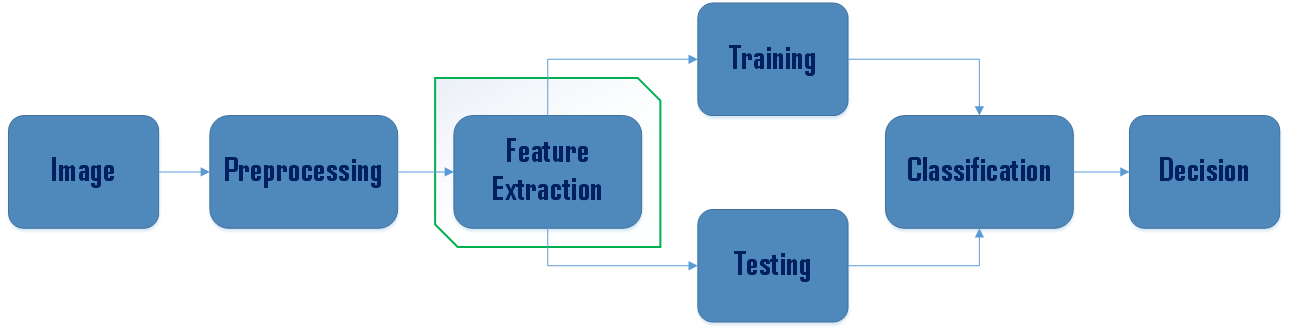
\includegraphics[width=\textwidth]{Pattern_Recognition_Framework.png}
	\caption{Overview of a generic facial recognition System}
	\label{fig:recog}
	
\end{figure} 

\noindent All these facts suggest that automatic recognition and analysis of human face allow many interesting applications in Biometrics, Human-Computer Interaction, and Security. From early 90's to till date, many researchers are working to find newer \& effective ways to derive features from human faces. As a result, more \& more ways of finding effective ways to extract features are coming in our way.\\
\linebreak
Deriving an efficient and effective feature representation is the fundamental component for any successful facial recognition system.
So, here our ongoing research aims to increase the robustness of the underlying feature descriptor against different factors.\\


%=======
\subsection{Problem Statement}
\noindent Here we want to create a system for facial feature extraction for expression detection. From the \figurename{ 1.1}, we can see that extracting information is the most important part of any facial feature extraction system. This face descriptor
should be robust in uncontrolled environment like noise, pose variation, illumination variation, aging, occlusion etc.\cite{ldpPaper}. So, designing a robust facial feature extractor is a critical task. Our aim is to create such a facial feature extractor which overcomes all of these obstacles.\\
\linebreak
Here is an image of all basic seven expressions in facial feature extractions.\\
\begin{figure}[h]
	\centering
	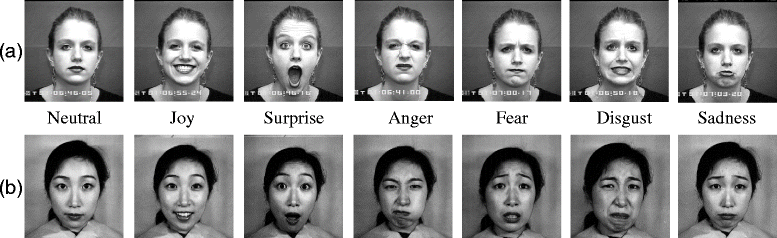
\includegraphics[width=\textwidth]{CKp_JAFFE.png}
	\caption{Different facial expressions from - (a) CK+ dataset and (b) JAFFE dataset}
	\label{sixExpressions}
	
\end{figure} 

A good feature representation should have the ability to
recognize all these expressions in all given environment.
%=======
\subsection{Research Challenges}
\label{sec:sec01}

All of the research works begins with some challenges. And for our case, it is also the same. Along with the data problems, there are also some issues which are appeared to be the research challenges such as-
\begin{itemize}
	\item variations in illumination
	\item occlusion
	\item facial alignments
	\item different facial poses
	\item aging
\end{itemize}

\subsubsection{Variations in illumination, pose, alignment}
\label{subsec:subsec01}
The first of the problems have come from the variation of illumination. Different illumination does not change the facial features, but it definitely changes the pixel values. And in digital image processing, everything depends on the pixel values.  \\
\linebreak
The alignment and pose of image subject can also affect the outcome. Overcoming these variations of illumination, pose and alignment is a major obstacle.\\

\subsubsection{Occlusion}
The meaning of the word 'Occlusion' means obstacle. Often there are some obstacles presented in the image. These sort of obstacles should be taken care of.

\subsubsection{Aging}
Age of the subject can also create variation in image data.\\

\noindent Human faces are non-rigid, dynamic objects with a large diversity in shape, color and texture. So a neat, robust, distinctive and effective descriptor is needed to extract facial features from a human face.

%#----


\subsection{Objectives}
Our thesis work focuses on achieving a Facial Feature Descriptor using directional micro-patterns which can provide better accuracy than the existing ones. Our thesis work will satisfy the following criteria :
\begin{itemize}
	\item Robust against illumination variations and random noise.
	\item Applicable in different face related problem domains, such as  facial expression analysis, face recognition, gender classification, age estimation and so on.
	\item Achieve superior performance in unconstrained environment than the existing state-of-the-art techniques.
	
\end{itemize}   
\noindent In the following chapter we will show the literates that have been analyzed and implemented by us.\\


\subsection{Contribution}
\noindent In this field of research, we have introduced a new facial feature extraction method which we are calling Adaptive Robust Local Complete Pattern
(ARLCP). In this method,  a new local pattern for effective facial feature representation using directional edge responses\cite{facialExpressions1} is introduced, which includes the description of the basic ARLCP operator and how to construct facial feature descriptor based on ARLCP. We effectively explore the advantage of edge response by incorporating the sign, magnitude and directional information that leads to more robust feature representation.\\

\subsection{Organization of the Thesis}
This thesis book has five chapters. Chapter 1 introduced about the facial feature representation system. Also the problem domain and research challenges of the system are also stated here. Chapter 2 gives us a overview of Related work on this
facial feature representation where we can get the idea of how far the research has
gone in this field. Chapter 3 describes our proposed face descriptor named Adaptive Robust Local Complete Pattern(ARLCP).Chapter 4 shows the analysis of different algorithms and comparative performance of our proposed feature descriptor. And finally in Chapter 5 we have referred to conclusion with some future plan for better facial feature representation. References are added at the end of this book.\\

\newpage
\section{Literature Review}
\label{chap:ch2}

To get some ideas about our field of work, we have gone through many research papers. In this chapter, we first present a discussion on different geometric and
appearance-based facial feature representation, which is followed by a review on
different local appearance-based methods. From there, we talk about various ideas and implementations that finally leads us to our final proposed method.\\
\subsection{Facial Feature Representation Methods}
\noindent In last two decades, many different methods have been proposed in the field of facial feature representation. Face recognition, expression detection and many other sectors are getting benefited from these representation methods. Here we divide these methods in two basic types - $i.$ Geometric feature-based methods  and $ii.$ Appearance-based methods.\\

\subsubsection{Geometric feature-based methods}
\noindent Geometric feature learning is a technique combining machine learning and computer vision to solve visual tasks\cite{wiki:geometry}. The feature vector is formed based on the
geometric relationships such as positions, angles or distances between different
facial components (eyes, ears, nose etc.). Many of the primitive facial recognition systems are mainly based on geometric feature-based methods.\\
\linebreak
\noindent In the beginning, facial action coding system (FACS)\cite{facs} was a
popular geometric feature-based method which represents facial expression with
the help of a set of action units (AU). Physical
behavior of a specific facial muscle is represented by each action unit. Then, a feature extraction method based on the geometric positions of 34 manually selected fiducial points is proposed by Zhang\cite{facialPoints}.A similar representation was adopted by Guo and Dyer\cite{gdGuo}. In that method, they
employed linear programming in order to perform simultaneous feature selection
and classifier training. In recent works in\cite{falscv} ,it has been found that geometric
features provide similar or better performance than appearance-based methods
in action unit recognition.\\
\linebreak
\noindent For face recognition, elastic bunch graph match (EBGM)\cite{ebgm} algorithm is the
most commonly-used geometric feature-based method. In this method, human
faces are represented as graphs, where nodes are positioned on fiducial points and
edges are labeled using distance vectors. A set of 16 geometric features for designing a gender
classification model is used by Brunelli
and Poggio\cite{Poggio_hyberbfnetworks} in which the features were extracted with HyperBF networks. Furthermore, a radial basis function (RBF) network and a
perceptron is experimented by Abdi et al.\cite{moreAboutmanWoman}. Here they achieved good classification result for both pixel-based inputs
and measurement-based inputs (geometric features). However, the effectiveness of geometric methods is heavily dependent on the
accurate detection of facial components, which is a difficult task in changing and
unconstrained environment, thus making geometric methods difficult to accommodate in many scenarios.

\subsubsection{Appearance Based Methods}
\noindent In appearance-based methods, the facial appearance is extracted by applying image filter or filter bank on the whole face image or some specific facial regions. Principal component analysis (PCA)\cite{cPadgetts}, independent component analysis (ICA)\cite{msBarlett,ccFA}, Gabor wavelets\cite{Yingli,mjLyons} and more recent
enhanced ICA (EICA)\cite{expFromVideo} are the commonly-used appearance-based methods for facial expression detections. Here, PCA is a global feature extraction method and  the
whole facial image is taken into account during feature vector generation. An optimal linear transformation from the original image space is provided
to an orthogonal eigenspace with reduced dimensionality in the sense of least mean
squared reconstruction error\cite{fcLBP}.\\
\noindent
\noindent The ``Eigenface" method was introduced by Turk and Pentland \cite{maTurk1991}. Later, linear discriminant analysis (LDA)\cite{discriminantAnalysis}, 2D PCA \cite{2DPCA}, local features analysis (LFA)\cite{LFA}, and dynamic link
architecture (DLA) \cite{DLA} methods were also investigated for feature representation
in face recognition systems. But their performance deteriorate in changing environment\cite{sobelLBP}. Donato et al.\cite{classifyFA} presented a comprehensive
analysis of different techniques for facial action recognition, which included PCA,
ICA, local feature analysis (LFA), Gabor wavelets, and local principal components (PCs). Among these techniques, ICA and Gabor wavelets provided the
best recognition rate. \\
\linebreak
\noindent In recent days, local appearance face descriptors based on local binary pattern
(LBP) \cite{fdLBP,fiaLBP} and its variants\cite{boosterFER} start to gain popularity. Local binary pattern is a
simple, yet effective local texture description technique, which is computationally efficient and robust against non-monotonic illumination variation. However, the LBP method performs weakly under the presence of large illumination
variation and random noise \cite{enhancedLTP1}, since a little variation in the gray level can easily
change the LBP code. Later, local ternary pattern (LTP) \cite{enhancedLTP1} was introduced to
increase the robustness of LBP in uniform and near-uniform regions by adding an extra intensity discrimination level and extending the binary LBP value to
a ternary code. Another method
named local directional pattern (LDP) \cite{robustFace} employed a different texture encoding
approach, where directional edge response values around a position is used instead
of gray levels. The motivation was to exploit more stable edge response values
instead of gray levels in order to encode the local texture, which increases the
robustness of the underlying feature descriptor.\\

\subsection{Local Texture Operators}

In this section, we present a review on some widely-used local pattern-based facial
feature descriptors. Here we divide these papers in three categories-
\begin{enumerate}
	\item \textbf{Basic Patterns:} 
	\begin{enumerate}
		\item Local Binary Pattern
		\item Local Binary Count
		\item Local Ternary Pattern
	\end{enumerate}
	\item \textbf{Complete Patterns:}
	\begin{enumerate}
		\item Complete Local Binary Pattern
		\item Complete Local Binary Count
		\item Complete Local Ternary Pattern
	\end{enumerate}
	
	\item \textbf{Adaptive Patterns:}
	\begin{enumerate}
		\item Adaptive Mean Binary Pattern
		\item Adaptive Robust Binary Count
		\item Directional Age Primitive Pattern
		
	\end{enumerate}
\end{enumerate} 

%=======
\subsection{Basic Patterns:}
\label{sec:sec01}
For our works of study, the Local Binary Pattern(LBP) and Local Ternary Patterns are considered to be the basic patterns. These methods are pretty straight-forward and the evolution of facial features extractions began with these methods.

\subsubsection{Local Binary Pattern(LBP)}




Local Binary Pattern(LBP) is considered to be one of the oldest and most used algorithms for facial feature extractions. This ground-breaking approach was introduced in 1996 by Ojala et al. \cite{lbp01} which forms labels for the image pixels by thresholding the 3 x 3 neighborhood of each pixel with the center value and considering the result as a binary number. The method is widely used for finding the texture pattern which helps to find the similarity
between two images.\\

In LBP method, some local neighbor values,$~P$ is taken around each pixel and generates
a P-bit binary code by thresholding the intensity value of the neighbour pixels
with respect to the intensity of the center pixel. The binary code of LBP is generated using equation  \ref{equation:2.1}.

\begin{equation}
LBP_{P,R}=\sum\limits_{p=0}^{P-1}{s({{g}_{p}}-{{g}_{c}}){{2}^{p}}}; 
\label{equation:2.1}
\end{equation}

\begin{figure}[h]
	\centering
	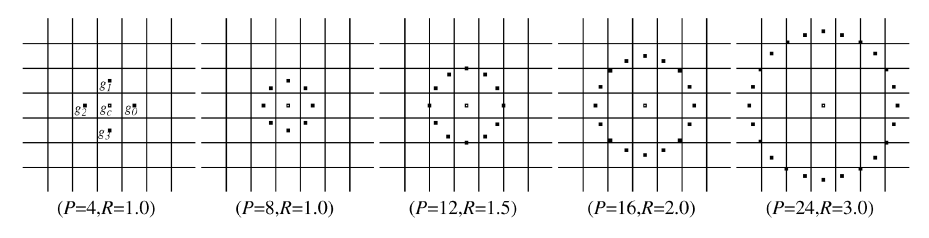
\includegraphics[width=\textwidth]{differentRadius}
	\caption{Circularly symmetric neighbor sets for different (P, R)}
	\label{figure:radius2}
\end{figure} 
Here, $g_c$ denotes the  value of a center pixel and $g_p$ defines the values of the local neighborhood pixels. $P$ is the number of the neighbors and $R$ is the radius of the neighbors as it is shown in figure \ref{figure:radius2}. If the function generates a value which is greater or equal to 1, it assigns a binary code ``1'' for the pixel, otherwise that pixel is assigned with the value 0 as it is stated in the equation \ref{equation:2.2}.

\begin{equation}
\tab  s(x)= 
\begin{cases}
1,& \text{if } x\geq 0\\
0,              & \text{otherwise}
\end{cases}
\label{equation:2.2}
\end{equation}

The generation of $P$-bit code is shown here in the figure \ref{figure:2.3} where $P=8$ and it takes a $3\times3$ region for applying the LBP method.

\begin{figure}[h]
	\centering
	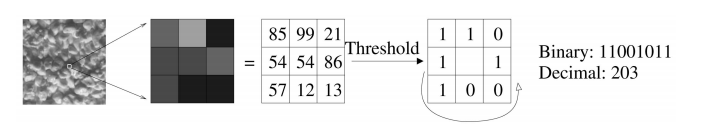
\includegraphics[width=.8\textwidth]{lbp_codes}
	\caption{The Basic LBP operator}%\cite{lbp04}}
	\label{figure:2.3}
\end{figure}


\subsubsection*{Limitations of LBP}
LBP is quick, easy and simple. But it is an intensity based operator. So noise can cause changes in the LBP code. As a result it will affect the performance and accuracy of the method. Generally, the presence of noise results in the decrease of accuracy and performance.\\

\subsubsection{Local Binary Count}
Local Binary Count (LBC)\cite{lbc01} is a variant of LBP. In the original LBP and its variants, each pixel in the local
neighbor set is turned to binary form by comparing it with the central
pixels and then are encoded to form the local binary
patterns. But in case of LBC, only the number of value 1's
in the binary neighbor sets are counted instead of encoding them. The following figure shows the working principles of LBC.
\begin{figure}[H]
	\centering
	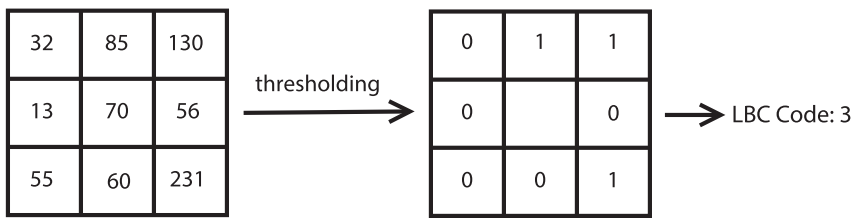
\includegraphics[width=0.8\textwidth]{lbc_new}
	\caption{Illustration of LBC (P = 8, R = 1)}
	\label{figure:illustratin of LBC}
\end{figure}
Here, the number of value 1's is
four in the binary neighbor set, thus the LBC code of the central pixel
is also three. We can define the computing process for the LBC as
follows:\\
\begin{equation}
LBC_{P,R}=\sum\limits_{p=0}^{P-1}{s({{g}_{p}}-{{g}_{c}})}; \tab  s(x)= 
\begin{cases}
1,& \text{if } x\geq 0\\
0,              & \text{otherwise}
\end{cases}
\label{equation:2.3}
\end{equation}

Like LBP, here also $g_c$ defines the center pixel intensity and $g_p$ defines the values of the local neighborhood pixels. $P$ is the number of the neighbors and $R$ is the radius of the local neighborhood. LBP and LBC mostly differed in the use of pixel values. In case of LBP, it uses the generated binary number to encode local patterns while the
LBC merely counts the number of value 1's in local neighbor set. Usually, LBP is mainly used for finding a structural information characterized by various patterns in the local neighbor while LBC focuses on finding the count of the pixels which are greater than the center one. Thus pixel positions can cause some effects in LBP but in case LBC, only the count of pixels that matters.\\


\begin{figure}[h]
	\centering
	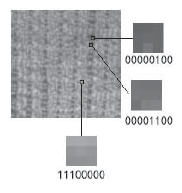
\includegraphics[width=0.5\textwidth]{lbc02}
	\caption{Schematic diagram of macroscopic textural structure that is quite
		different from the micro-structure.}
	\label{figure:2.4}
	
\end{figure}
In statistical texture analysis methods, the repeats for a large number of local microcosmic patterns are regarded to be the microscopic structures. The whole structure can be characterized using the statistics of the selected local microcosmic patterns which are quite different from the macroscopic textural structure. In the figure \ref{figure:2.4}, the micro-structures, $``00000100"$ and $``00001100"$, may
be contained in a macroscopic ``line" in texture image, and a
micro-structure ``line" which is $``11100000"$ may be a ``spot" in the
image. That is a macroscopic  textural structure in the real image which
may consist of many different local binary micro-structures. Different macroscopic textural structures may have similar micro-structures, but can different in frequencies of occurrence. According to Ojala et al. in 2002\cite{lbp02}, the
local binary pattern can characterize the local texture effectively
by detecting ``micro-structure" . The LBP
characterizes the distribution of local pixels effectively by using the
local binary encoding but cannot detect the frequency of occurrences. This is where LBC comes in handy as it can distinguish the different distributions of local pixels. Thus the LBC features can also represent
the macroscopic textural structures.
\subsubsection*{Limitations of LBC}
LBC depends of the count of the pixels. As a result, it can generate same codes for different positional patterns which may cause errors in local structural patterns. \\

\subsubsection{Local Ternary Pattern :}

Local binary pattern (LBP) is very sensitive to noise. Local ternary pattern (LTP) partially solves this problem by encoding the small pixel difference into a third state. Local Ternary Pattern (Tan and Triggs, 2010)\cite{ltp02} introduces one additional discrimination level than LBP.  the
pixel difference between the center pixel and the neighboring
pixel was encoded into a trinary code.

\begin{equation}
LTP_{P,R}=\sum\limits_{p=0}^{P-1}{s({{g}_{p}}-{{g}_{c}}){{2}^{p}}}; \tab  s(x)= 
\begin{cases}
1,&  x\geq t\\
0,&  -t < x <t\\
-1,&  x<-t
\end{cases}
\label{equation:2.4}
\end{equation}

Here in the equation \ref{equation:2.4},  $g_c$ defines the center pixel intensity and $g_p$ defines the values of the local neighborhood pixels. $P$ is the number of the neighbors and $R$ is the radius of the local neighborhood. ``t'' here defines a user defined threshold. Thus this 3-valued code is more resistant to noise, but it is no longer strictly invariant to gray level transformations. Here is an illustration of LTP where the threshold is set to 5\cite{ltp03}.

\begin{figure}[h]
	\centering
	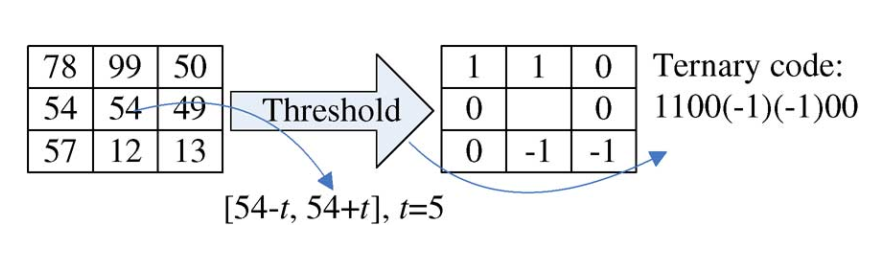
\includegraphics[width=\textwidth]{ltp_code1}
	\caption{Illustration of the basic LTP operator}
	\label{figure:2.7}
\end{figure}  

When using in equation \ref{equation:2.4} a $3^n$ valued code is generated but the uniform pattern argument are needed to be applied here. Thus it is desirable to reduce its dimensionality\cite{ltp01}. So, the experiment below uses a coding
scheme that splits each ternary pattern into its positive and negative halves as illustrated in figure \ref{figure:2.8} which are subsequently treated with two different LBP descriptors for which separate
histograms and similarity metrics are computed, combining the
results only at the end of the computation\cite{enhancedLTP1}.

\begin{figure}[h]
	\centering
	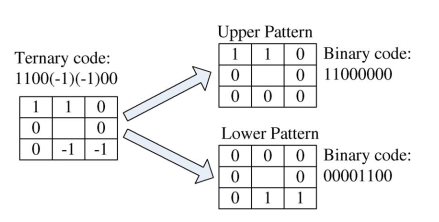
\includegraphics[width=\textwidth]{ltp_code2}
	\caption{Illustration of the basic LTP operator}
	\label{figure:2.8}
\end{figure}  
\subsubsection*{Limitations of LTP}
Though LTP performs better than LBP, it is still susceptible to noise and illumination variations as it employs simply the gray level values.

\subsection{Complete Patterns:}
Complete patterns are a fusion of a few image components.
Instead of the total intensity of the image, here the value comparison of sign, magnitude of difference between center and neighbors and the center intensity value is used. All these values should provide more robustness to the descriptors.

\subsubsection{Complete Local Binary Pattern:}
The completed
LBP (CLBP) descriptor was proposed by Guo et al.\cite{clbp01}
in order to improve the performance of LBP descriptor. Simple LBP techniques are good for showing local image features. Also there is a magnitude component in images which may contribute
additional discriminant information if it is properly used. Moreover, there are a lot of potential uses of the center pixel value of the picture\cite{Varma2003}. So, CLBP combines all these three components to make a more robust descriptor.
\begin{figure}[h]
	
	\centering
	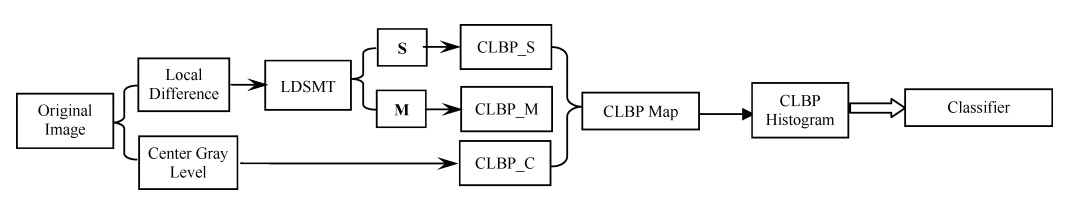
\includegraphics[width=\textwidth]{clbp_frameWorkPaper}
	\caption{Framework of CLBP}
	\label{figure:clbp1}	
\end{figure}
From figure \ref{figure:clbp1}, we can see that, the local difference in the image is converted into Sign(S) and Magnitude(M) values which are here denoted as CLBP\_S and CLBC\_M. The center pixel(C) is also used which is denoted here by CLBP\_C. Then all these three codes are combined to create CLBP histogram which can be used for texture classifications.\\
\linebreak
Here  CLBP\_S is created using the same equations from the LBP method.
\begin{equation}
CLBP\_S_{P,R}=\sum\limits_{p=0}^{P-1}{s({{g}_{p}}-{{g}_{c}}){{2}^{p}}}; \tab  s(x)= 
\begin{cases}
1,&  x\geq 0\\
0,&  \text{Otherwise}
\end{cases}
\label{equation:2.5}
\end{equation}
But as the magnitude components are not binary like $``1"$ or $``-1"$, rather they are continuous values. So, in order to code for magnitude values, the CLBP\_M operator is calculated using:
\begin{equation}
CLBP\_M_{P,R}=\sum\limits_{p=0}^{p-1}{t(m_p,c){{2}^{p}}}; \tab  t(x,c)= 
\begin{cases}
1,&  x \geq c\\
0,&  \text{Otherwise}
\end{cases}
\label{equation:2.6}
\end{equation}
in this equation, $c$ is a threshold to be determined adaptively as the mean value of the whole image. $m_p$ is the magnitude of difference between center \& neighbor pixels.  Both of these CLBP\_S and CLBP\_M produce binary string so that they can be conveniently used together for pattern classification using concatenation. \\
\linebreak
The third operator is the CLBP\_Center  which is defined here by :
\begin{equation}
CLBP\_C_{P,R} = t(g_c,c_1)
\label{equation:2.7}
\end{equation}
where t is defined in equation \ref{equation:2.6} and $c_1$ is set as the average gray level of the whole image. All of these three components are combined to create a histogram which works as the feature descriptor.
\subsubsection*{Limitations of CLBP}
Though CLBP is better than LBP, it performs weakly under the presence of random noise and large illumination variation as it uses the direct intensity values like LBP.\\

\subsubsection{Complete Local Binary Count(CLBC)}
Similar to CLBP,  LBC is extended to completed
LBC (CLBC) which is proposed in\cite{clbc01}. This procedure is also devided into three operators :  CLBC-Sign(CLBC\_S), CLBC-Magnitude(CLBC\_M) and   CLBC-Center(CLBC\_C). These operators can be combined into joint or hybrid distributions and they are used for rotation invariant texture classification.\\
\linebreak
Here CLBC\_S is basically the basic LBC descriptor. 
\begin{equation}
CLBC\_S_{P,R}=\sum\limits_{p=0}^{P-1}{s({{g}_{p}}-{{g}_{c}})}; \tab  s(x)= 
\begin{cases}
1,&  x\geq 0\\
0,&  \text{Otherwise}
\end{cases}
\label{equation:2.10}
\end{equation}
the meaning of $g_c$, $g_p$, $P$ \& $R$ is stated in the equation \ref{equation:2.3}. The CLBC\_M counts how
many neighbors have comparatively much higher intensity than the
center pixel which is used to extract local intensity differences.
\begin{equation}
CLBC\_M_{P,R}=\sum\limits_{p=0}^{P-1}{t(m_p,c)}; \tab  t(x,c)= 
\begin{cases}
1,&  x\geq c\\
0,&  \text{Otherwise}
\end{cases}
\label{equation:2.11}
\end{equation}
the values of $m_p$, $c$ are stated in the equation \ref{equation:2.6}. Also according to \cite{enhancedLTP1}, the center pixel can be used to express the local gray level in the image which is expressed in CLBC\_C.
\begin{equation}
CLBC\_C_{P,R} = t(g_c,c_1)
\label{equation:2.12}
\end{equation}
As we can see, it is pretty similar to equation no. \ref{equation:2.7}. Similarly using the count of the pixels, three different histograms are generated which are finally used as the feature descriptor.Thus CLBC discards the structural information from LBP operator and only concentrate on local binary gray-scale difference.

\subsubsection*{Limitations of CLBC}
It may generate same codes for different pixels as it only counts the total number of 1s rather than the position like LBC.\\%=========================================================

\subsubsection{Complete Local Ternary Pattern(CLTP)}
Complete Local Ternary Pattern(CLTP) (T. H. Raseen \& B. E. Khoo, 2013)\cite{cltp01} extends the concept of LTP \& its framework is similar to CLBP. It capitalizes the ternary pattern system of LTP and thus for local difference of the image, the value of sign and magnitudes are decomposed into two complementary components as follows : 
$$
s_p^{upper} = s(i_p - (i_c + t)), \tab s_p^{lower} = s(i_p - (i_c - t))\\
$$
$$
m_p^{upper} = |i_p - (i_c +t)| \tab 	m_p^{lower} = |i_p - (i_c -t)|\\
$$
Here $i_c$ defines the intensity of the center pixel where $i_p$ shows the intensity value of $p_{th}$ pixel. $t$ is the user defined threshold for the image. For CLTP\_Sign, the $	s_p^upper$ and $s_p^lower$ are used to build the $CLTP\_S_{P,R}^{upper}$ and $CLTP\_S_{P,R}^{lower} $ respectively.
\begin{equation}
CLTP\_S_{P,R}^{upper} = \sum\limits_{p=0}^{P-1}{s(i_p - (i_c + t){{2}^{p}}}; \tab  	s_p^{upper}= 
\begin{cases}
1,&  i_p\geq i_c + t\\
0,&  \text{Otherwise}
\end{cases}
\end{equation}

\begin{equation}
CLTP\_S_{P,R}^{lower} = \sum\limits_{p=0}^{P-1}{s(i_p - (i_c - t){{2}^{p}}}; \tab  	s_p^{lower}= 
\begin{cases}
1,&  i_p < i_c - t\\
0,&  \text{Otherwise}
\end{cases}
\end{equation}

The $CLTP\_S_{P,R}$ is the concatenation of the $CLTP\_S_{P,R}^{upper}$ and the $CLTP\_S_{P,R}^{lower}$ which is as follows:
\begin{equation}
CLTP\_S_{P,R}= [CLTP\_S_{P,R}^{upper},CLTP\_S_{P,R}^{lower}]
\end{equation}

In the similar way , $CLTP\_M_{P,R}$ is built using the two magnitudes of $	m_p^{upper}$ and $	m_p^{lower}$ as  follows:
\begin{equation}
CLTP\_M_{P,R}^{upper} = \sum\limits_{p=0}^{P-1}{t(m_p^{upper},c){{2}^{p}}}; \tab  	t(m_p^{upper},c)= 
\begin{cases}
1,&  |i_p -(i_c + t)\geq c\\
0,&  \text{Otherwise}
\end{cases}
\end{equation}

\begin{equation}
CLTP\_M_{P,R}^{lower} = \sum\limits_{p=0}^{P-1}{t(m_p^{lower},c){{2}^{p}}}; \tab  	t(m_p^{lower},c)= 
\begin{cases}
1,&  |i_p -(i_c - t)\geq c\\
0,&  \text{Otherwise}
\end{cases}
\end{equation}
\begin{equation}
CLTP\_M_{P,R}= [CLTP\_M_{P,R}^{upper},CLTP\_M_{P,R}^{lower}]
\end{equation}
Here $i_c$ ,$i_p$ $P$, $R$ and $t$ is defined before. Finally, the third component which involved the center pixel value is mathematically described as follows:
\begin{equation}
CLTP\_C_{P,R}^{upper} = t(i_c^{upper},c_I),\\
CLTP\_C_{P,R}^{lower} = t(i_c^{lower},c_I),
\end{equation}

where $i_c^{upper} = i_c + t$, $i_c^{lower} = i_c - t$ and $c_I$ is the average gray level of the whole image. After getting all these three histograms, these are combined to create the feature vectors in CLTP.
\subsubsection*{Limitations of CLTP}
As it uses the same concept of LTP, it is susceptible to noise and illumination variations.\\

\subsection{Adaptive Patterns}
In this category, methods with adaptive thresholding are only going to be discussed.
\subsubsection{ Adaptive Median Binary Pattern(AMBP)}
Adaptive Median Binary Pattern (AMBP) is variation of Median Binary Patterns(MBP) operators which uses an adaptive thresholding. The MBP operator maps from the intensity space to create a binary pattern by thresholding the pixels against their median value within a neighborhood. According to \cite{ambp01}, the MBP at pixel $(i,j)$ is given in figure \ref{figure:MBP1} using 

\begin{equation}
MBP(i,j)=\sum\limits_{k=0}^{L-1}{{{2}^{k}}H(b_k-\tau)}; \tab H(b)=
\begin{cases}
1,&  b\geq 0\\
0,&  \text{Otherwise}
\end{cases}
\label{equation:2.13}
\end{equation} 
Here b is the intensity of $b^{th}$ pixel and $H$ is the Heaviside unit step function which is also referred to be binary thresholding function. $L$ is the patch size and $\tau$ is considered to be the constraining threshold which is the median value in case of MBPs.
\begin{figure}[H]
	\centering
	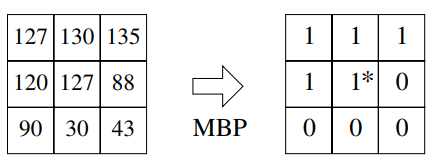
\includegraphics[width=0.8\textwidth]{mbp}
	\caption{MBP operator for 3X3 patches}
	\label{figure:MBP1}
\end{figure}
In figure \ref{figure:MBP1}, an MBP operator for a $3 \times 3$ patch (i.e. L = 9) with a median value
of 120 (i.e. $\tau = 120$) is used. Output binary pattern of  MBP = ${100011110}_2$ = $286$.
Ordering of bits in the binary pattern uses $b_0$ as the least significant bit which is shown in the following figure \ref{figure:following} :

\begin{figure}[H]
	\centering
	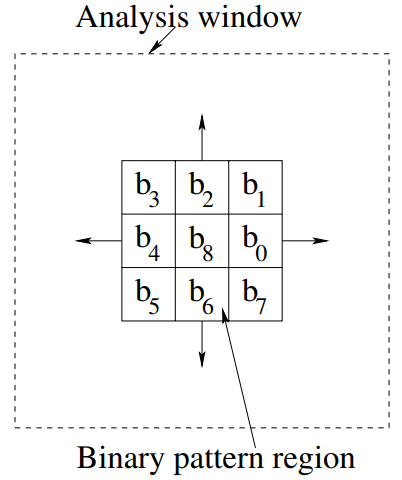
\includegraphics[width=0.4\textwidth]{ambp_ref}
	\caption{Illustration of AMBP terminology}
	\label{figure:following}
\end{figure}
However, a small windows can miss a lot of information and also a larger window can be sometimes bad for performances. Thats is why, AMBP considers larger and adaptive analysis windows to compute optimal local threshold.\\
\begin{equation}
AMBP(P,R)=\sum\limits_{p=0}^{P-1}{{{2}^{k}}s(g_p-\tau)} \tab  s(x)= 
\begin{cases}
1,&  x\geq 0\\
0,&  \text{Otherwise}
\end{cases}
\label{equation:2.15}
\end{equation}

Here in the equation \ref{equation:2.15}, $P$ is defined as the patch size. The values of $g_p$, $\tau$ and $s(x)$ are described in previous equations. In the AMBP algorithm from algorithm 1 where, $S$ is the square region around a pixel, $k_{max}$ is the maximum analysis window. The median, minimum and maximum value inside $S$ is stated by $Z_{med}$,$Z_{min}$ and $Z_{max}$ respectively.
\begin{algorithm}
	$\text{\textbf{Input : }Gray scale Image} I; \text{maximum analysis window }k_{max}; \text{patch size} L = 9$\;
	$\text{\textbf{Output:} Adaptive Median Binary Pattern Image}, M$\;
	\For {$\text{\textbf{all }} i,j$}
	{
			$k \gets 1$ \;
			\Repeat{ $k \leq k_{max}$}
			{
					$S \gets I[i-k:i+k, j-k : j+k]$ \;
					$Z_{med} \gets \text{median(S)}$ \;
					$Z_{min} \gets \text{min(S)}$\;
					$Z_{max} \gets \text{max(S)}$\;
					\If{$Z_{min} < 	Z_{med} <	Z_{max}$}{break}
					$k \gets k+1$ \;	
			}
		\If{$Z_{min} < 	I[i,j] <	Z_{max}$}
		{$\tau = I[i,j]$}
		\Else{$\tau = Z_{med}$}
		$M[i,j] \gets L-\text{bit binary pattern using } \tau \text{ and Equation } \ref{equation:2.15}$
			\label{algo:1}		
	}

	\caption{Adaptive Median Binary Patterns(AMBP)}
\end{algorithm}

\subsubsection*{Limitations}
AMBP is sensitive to noise as it uses the intensity values like LBP.\\

\subsubsection{Adaptive Robust Binary Pattern(ARBP)}
Adaptive Robust Binary Pattern(ARBP) (X. Wu et al. 2018)\cite{arbp01} follows the similar concepts as LBP \& AMBP. It contains three steps - determination of the optimal size of the analysis window, determination of the local threshold value and encoding.

In contrast to AMBP, here a new parameter is introduced $Z_{para}$ that is used to generate the threshold $\tau$. This parameter can be selected from $Z_{ave}$ and $Z_{med}$ whichever has the furthest distance from the center pixel. Also, here $Z_{ave}$ defines the average intensity. The equation of ARBP is given here
\begin{equation}
ARBP(P,R)=\sum\limits_{p=0}^{P-1}{{{2}^{k}}s(g_p-\tau)} \tab  s(x)= 
\begin{cases}
1,&  x\geq 0\\
0,&  \text{Otherwise}
\end{cases}
\label{equation:2.20}
\end{equation}
Here the value of $s$, $g_p$ and $x$ is already defined in the equation \ref{equation:2.15} but threshold $\tau$ is calculated differently in the Algorithm 2. The algorithm for ARBP is given down here which shows the step by step guide for the descriptor.\\
\begin{algorithm}[H]
	$\text{\textbf{Input : }Gray scale Image}~ I; \text{maximum analysis window }k_{max}; \text{patch size} L = 9$\;
	$\text{\textbf{Output:} Adaptive Robust Binary Pattern Image}, M$\;
	\For {$\text{\textbf{all }} i,j$}
	{
		$k \gets 1$ \;
		\Repeat{ $k \leq k_{max}$}
		{
			$S \gets I[i-k:i+k, j-k : j+k]$ \;
			$Z_{med} \gets \text{median(S)}$ \;
			$Z_{min} \gets \text{min(S)}$\;
			$Z_{max} \gets \text{max(S)}$\;
			$Z_{ave} \gets \text{average(S)}$\;
			$ d =\frac{1}{|S|}\sum\limits_{m\epsilon S(i,j)}{x_c - x_m}, m \neq c$\;
			\If{$|Z_{med} -I[i,j]|  <|Z_{ave} -I[i,j]|$}{$Z_{para}=Z_{ave}$\;}
			\Else{$Z_{para}=Z_{med}$\;}
			\If{$Z_{min} + \alpha . d <Z_{para}<  Z_{max} - \alpha.d $}{break}
			$k \gets k+1$ \;	
		}
		\If{$Z_{min} + \alpha.d < 	I[i,j] <	Z_{max} -\alpha.d$}
		{$\tau = I[i,j]$}
		\Else{$\tau = Z_{para} (\tau \text{ is the parmater used as the threshold}) $}
		$M[i,j] \gets L-\text{bit binary pattern}$	
	}
	\caption{Adaptive Robust Binary Pattern(ARBP)}
\end{algorithm}

\subsubsection*{Limitations}
It does better job than AMBP but still noise can affect its performance.\\


\subsubsection{Directional Age Primitive Pattern(DAPP)}
DAPP(M. T. B. Iqbal et al., 2017)\cite{dapp01} efficiently represents both cranio-facial growth(shape) \& skin aging (texture) information.
Initially 3 states are considered- (1) is set for Wrinkle textures, (2) is set for lip/eye corners, otherwise it is set to 0 as:\\

\begin{equation}
P_{init}(x,y)= 
\begin{cases}
1,& \text{if } \text{$\theta$ = $\tau_1$}\\
2,& \text{if } \text{$\theta$ = $\tau_2$}\\
0,              & \text{otherwise}
\end{cases}
\end{equation}
\vspace*{.7cm}

\noindent Here, $\tau_1$ refers to 45$^\circ$ and $\tau_2$ refers to  90$^\circ$ as shown in figure \ref{fig:dapp_all}.  
\begin{figure}[H]
	\begin{center}
		\centering
		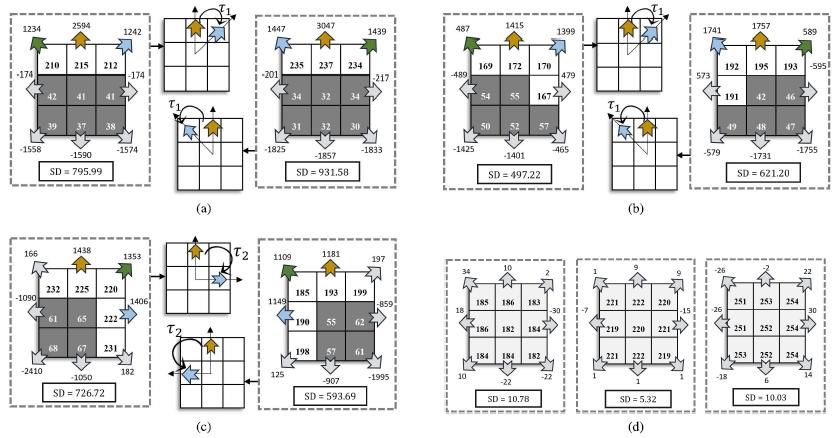
\includegraphics[width=\textwidth]{dapp_all.png}
		\caption{(a). Straight wrinkle (b) Curved Wrinkle (c) Eye corner (d) Flat patch}
		\label{fig:dapp_all}
	\end{center}
\end{figure}
Wrinkles can appear either as straight edges as in \ref{fig:dapp_all}(a) or curved edges as shown in figure \ref{fig:dapp_all} (b). Moreover, secondary and tertiary edge response can be clockwise or counter clockwise to each-other. All these information extends these three categories into six as equation \label{eqn:six}.\\

\begin{equation}
s(x)= 
\begin{cases}
1,&~ if,~ Diff_{ST}< \gamma\\
2,&~ if,~ Diff_{ST}\geq \gamma,~dir_1 \circlearrowleft dir_2\\
3,&~ if,~ Diff_{ST}\geq \gamma,~ dir_1 \circlearrowright dir_2\\
4,&~ if,~ dir_1 \circlearrowleft dir_2\\
5,&~ if,~ dir_1 \circlearrowright dir_2\\
0,&~ if,~ P_{init}=0\\
\end{cases}
\label{eqn:sixtimes}
\end{equation}

\iffalse
\[
P= \begin{cases}
1,& \text{if } \text{Diff$_ST$ < $\gamma$}\\
2,& \text{if } \text{Diff$_ST$ $\geq$ $\gamma$, dir_2  dir$_1$}\\
3,& \text{if } \text{Diff$_ST$ $\geq$ $\gamma$, dir$_2$  dir$_1$}\\
4,& \text{if }  \text{dir$_2$  dir$_1$}\\
5,& \text{if }  \text{dir$_2$  dir$_1$}\\
0,& \text{otherwise}
\end{cases}
\]
\fi

\noindent Threshold is generated as the highest accumulated bin of histogram of Standard Deviation (SD) of edge responses in cheek region. DAPP code generation is shown in figure \ref{fig:dapp_code_generation}



\begin{figure}[H]
	\begin{center}
		\centering
		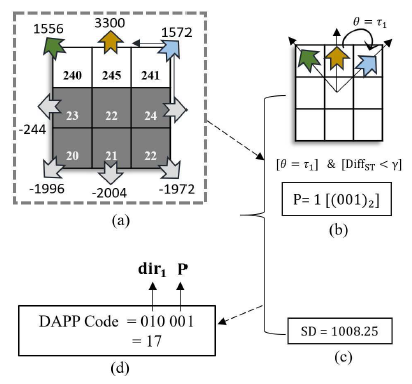
\includegraphics[width=0.7\textwidth]{dapp_code_generation.png}
		\caption{(a). Sample image patch and its Kirsch responses. (b) Age-Primitive code computation (c) Adaptive Thresholding (d) Final DAPP computation}
		\label{fig:dapp_code_generation}
	\end{center}
\end{figure}


\noindent Here in figure \ref{fig:dapp_code_generation}, Kirsch masks are applied to get eight directional edge response. Then top three edge responses are selected as primary, secondary and tertiary edge response. Then final age-primitive code, P is generated using equation \ref{eqn:sixtimes}. Here angle between primary and secondary edge response is 45$^\circ$, so $\theta$ is $\tau_1$ here. Difference between secondary and tertiary edge response is assumed to be less than the threshold $\sigma$. Therefore, final age-primitive code, P is 1 for this example. Then the direction of primary edge response and final age-primitive code is concatenated to generate final DAPP code that is 17 in this case.


\newpage
\section{ Proposed Feature Descriptor: Adaptive Robust Local Complete Pattern (ARLCP)}



\subsection{ Overview }
%					\begin{flushleft}
The recent challenge in facial expression recognition systems is to extract facial features which are robust in changing environment. In this chapter, we explain the proposed Adaptive Robust Local Complete Pattern (ARLCP), a new local pattern for effective facial feature representation, which includes the description of the basic ARLCP operator and how to construct facial feature descriptor based on ARLCP.



In our approach, we take images from datasets and then divide the images into $n \times n$ (e.g. $5 \times 5$,  $10 \times 10$) regions. For each of the regions, we extract features and then create feature vector. Later on, we concatenate each of the vectors to generate final feature vector that represents an image. 





%					\end{flushleft}	
\subsection{Adaptive Robust Local Complete Pattern (ARLCP) Code}



LBP, LTP and LBC methods use merely the gray level intensity values to encode the local texture of an image, which makes these methods unstable under the presence of large illumination variations. LBP is also susceptable to noise. Therefore, some recent local pattern operators exploit more stable gradient information or edge response values instead of gray levels. One such method is the Sobel-LBP that combines the LBP with the Sobel operator in order to enhance the local features and thus facilitates the extraction of more detailed information. Another approach is the local directinal pattern (LDP) [6] that employs eight directional edge response values to encode the local texture. However,
since both Sobel-LBP and LDP methods use two discrimination levels (0
and 1) to generate binary texture patterns, these methods tend to produce inconsistent codes in uniform and smooth regions, where the intensity variations among the neighbors are negligible. Also LDP dose  not consider the magnitude of edge response. Another approach is the idea of completeness in micro-pattern considering the sign and magnitude of local difference along with the center intensity value. Such type of methods like CLBP, CLBC and CLTP still use the gray level intensity values which are susceptible to noise. Considering these limitations, we present the Adaptive Robust Local Positional Pattern (ARLCP) - a new local texture pattern for representing facial features. Instead of quantizing the gray level intensities like CLBP or CLTP, the ARLCP operator encodes the more stable edge esponse values of a local neighborhood, which retains more information of the local image content. Additionally, the proposed method uses adaptive threshold instead of a static one for each image as static threshold on primary response is quite sensitive since it may wipe-out either edge pixels in low-contrast image or flat pixels in natural noisy images


\subsection{The Basic ARLCP Encoding Scheme}
\begin{figure}[H]
	\begin{center}
		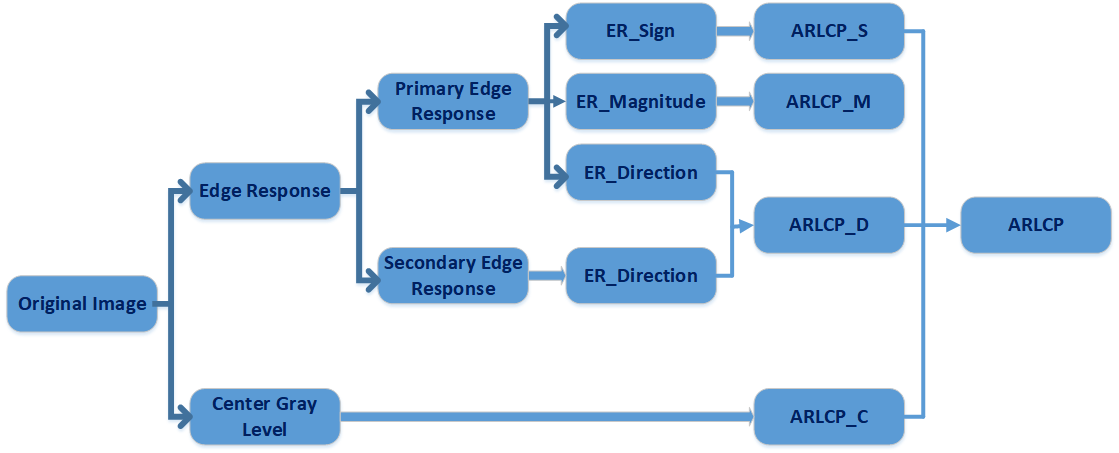
\includegraphics[width=12cm,height=8cm,keepaspectratio]{ARLCP_Framework.png}
		\caption{ARLCP Framework}
				\label{fig:ARLCP_Framework}
	\end{center}
\end{figure}
Here we propose a face descriptor, Adaptive Robust Local Complete Pattern (ARLCP) as shown in figure \ref{fig:ARLCP_Framework}, for generating feature representation of facial images which is robust in presence of noise and illumination variation. In the preprocessing step an image is first cropped based on the position of the eyes, nose and mouth and the face descriptor is applied on the resulting cropped image to generate a face representation. In our proposed method, we follow four steps to compute ARLCP feature vector:
\begin{enumerate}[i.]
	\item Edge response computation
	\item Primary and secondary edge response selection
	\item Threshold($\sigma$) generation
	\item Sign, Magnitude, Direction and Center codes generation
	\item Histograms of Sign, Magnitude, Direction and Center codes generation 
\end{enumerate}

\subsubsection {Step 1: Edge Response Computation }
To get direction information of each pixel, we extract edge response values in eight different directions. We apply Kirsch compass mask shown in figure \ref{fig:KirschMask} for this purpose since it detects different directional edge responses more accurately than the others due to the consideration of all eight neighbors. We convolve the Kirsch mask in eight different orientations by rotating $45^\circ$
where, I(x, y) is the pixel value, K$_i$ is the i$^{th}$ Kirsh mask among eight (K$_0$, K$_1$, ...K$_7$), as shown in \ref{fig:KirschMask}. ER$_i$ is their corresponding edge response values as shown in figure \ref{fig:apply_mask}.
\begin{figure}[H]
	\begin{center}
		\centering
		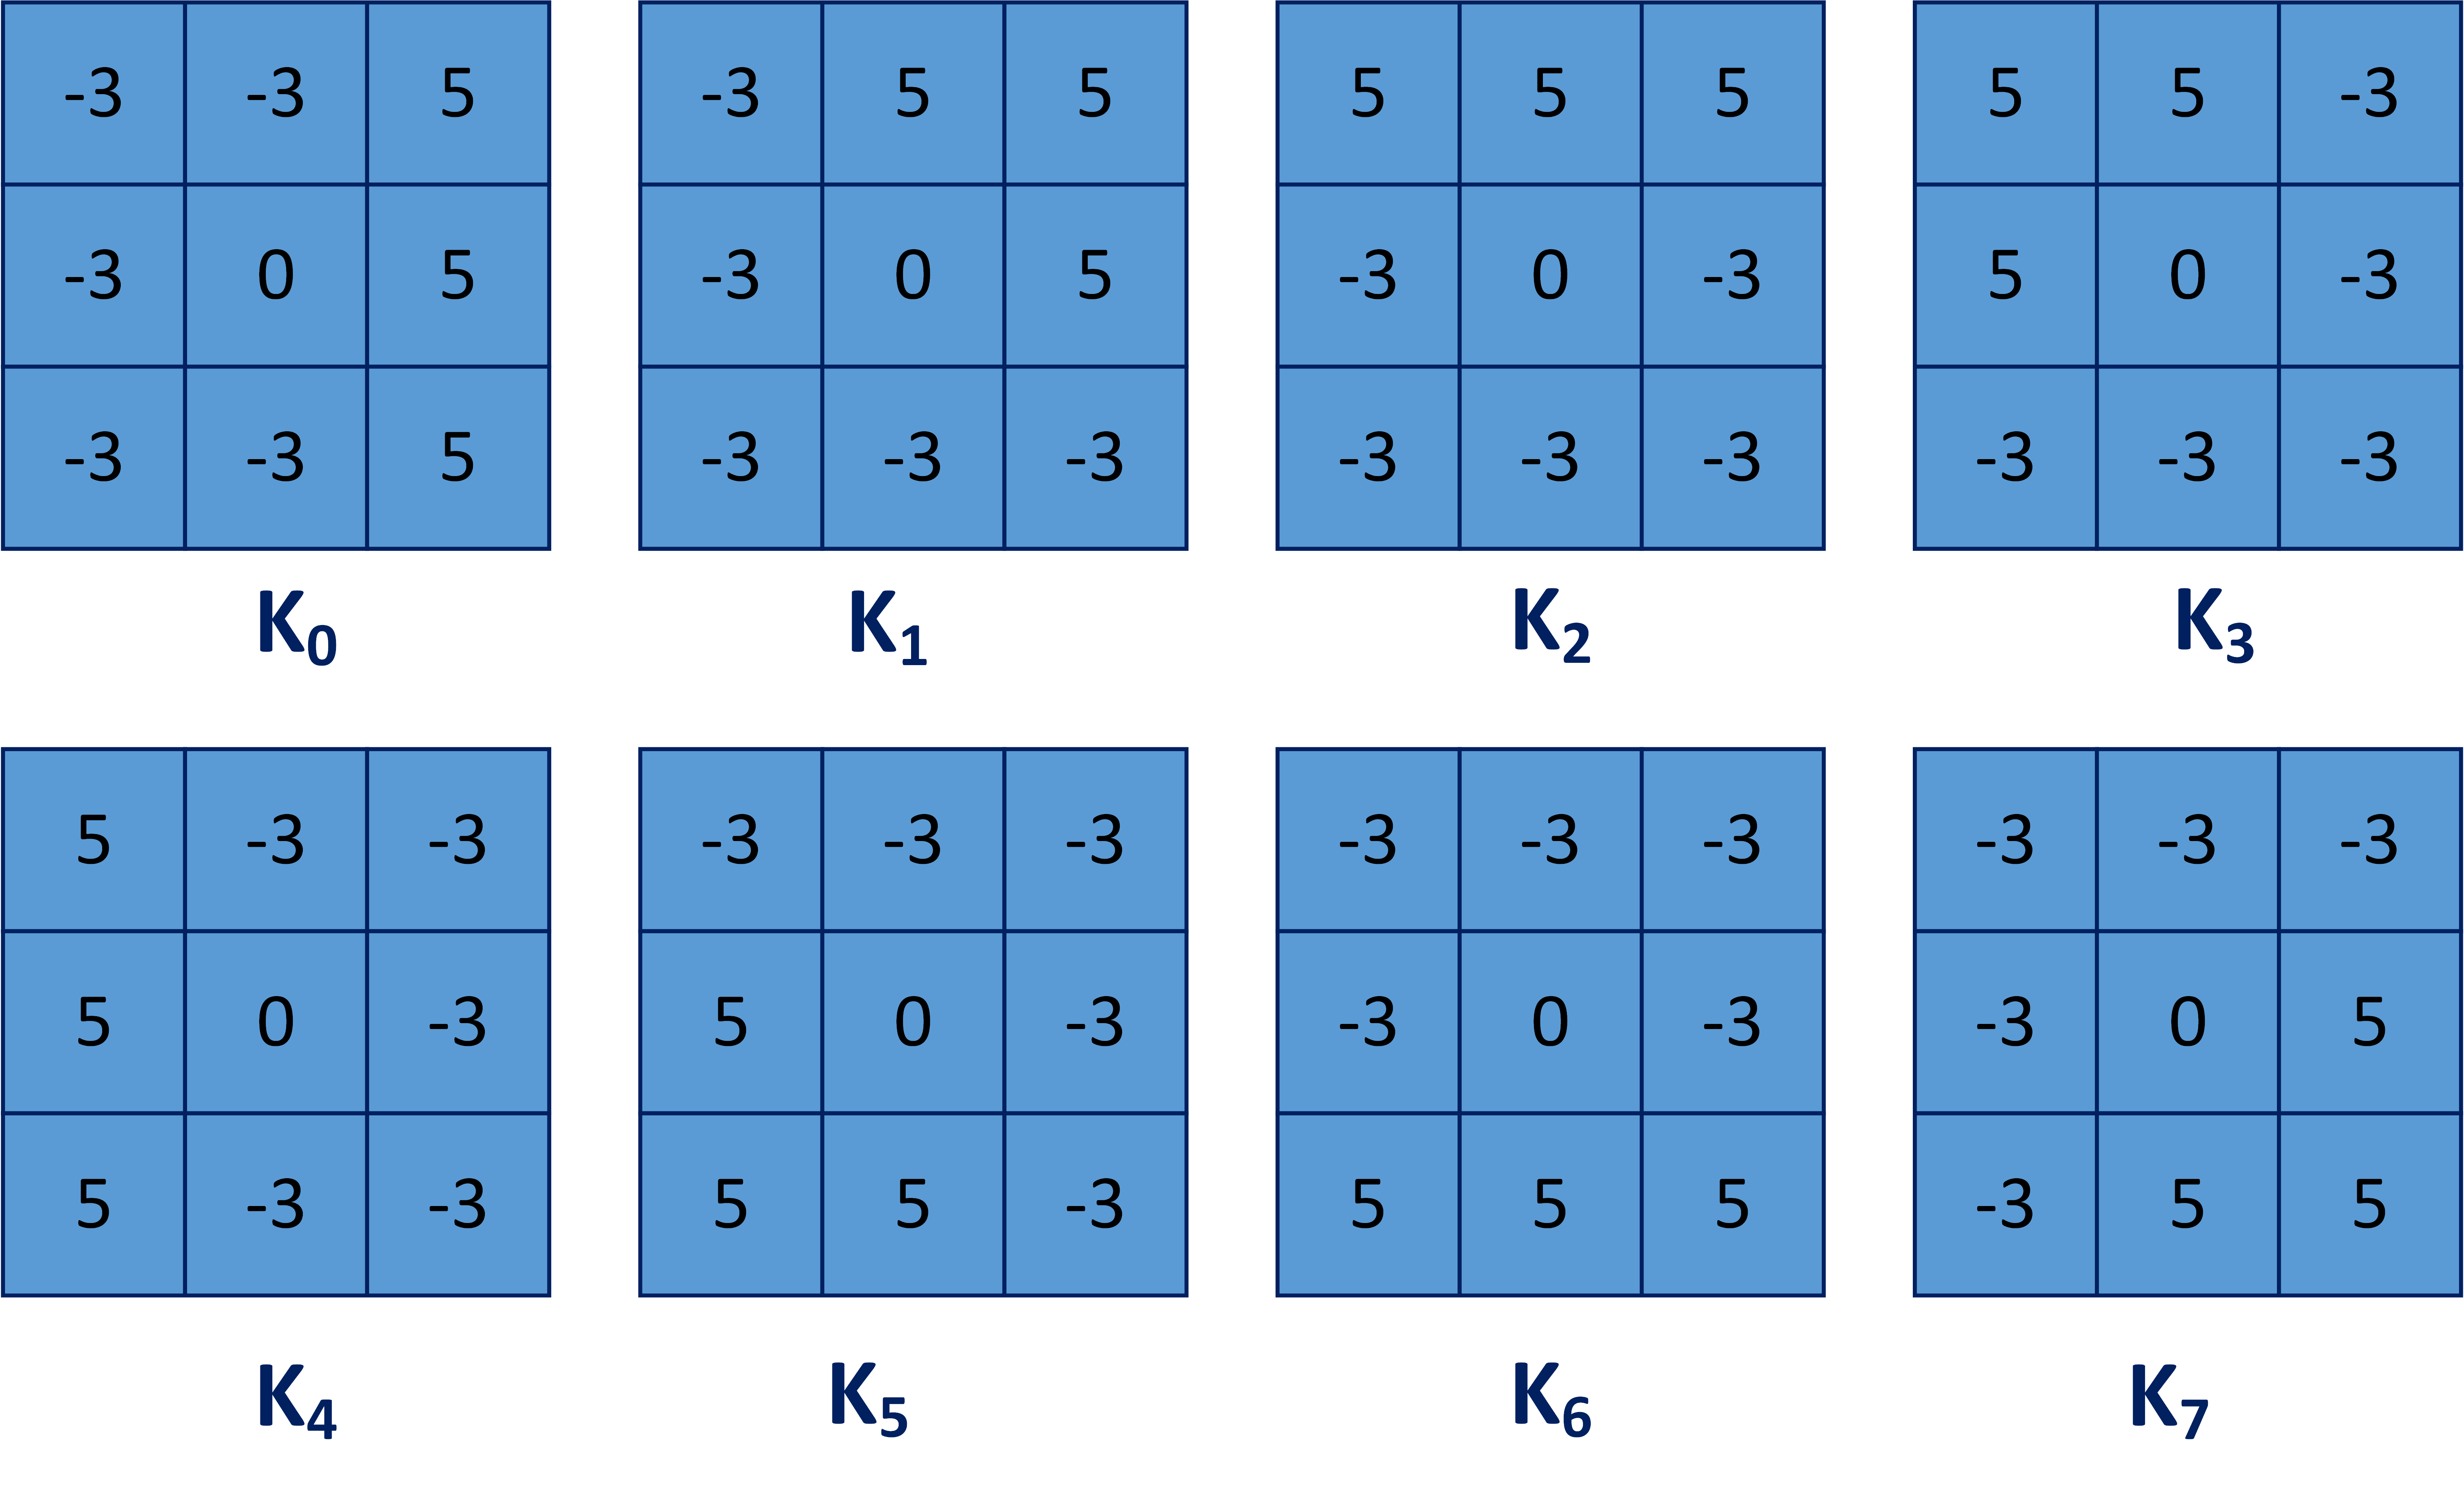
\includegraphics[width=0.7\textwidth]{KirschMask.png}
		\caption{Kirsch Mask}
				\label{fig:KirschMask}	
	\end{center}
\end{figure}

\begin{figure}[H]
	\begin{center}
		\centering
		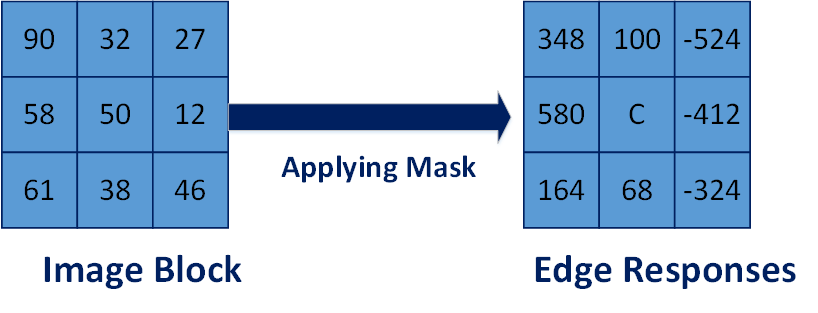
\includegraphics[width=0.7\textwidth]{apply_mask.png}
		\caption{Edge Responses}
				\label{fig:apply_mask}
	\end{center}
\end{figure}


\subsubsection{Step 2: Primary and secondary edge response selection} 	
Applying the 8 masks generates 8 responses each representing the edge significance in its respective direction. Among these eight edge responses, we consider two top most edge responses as they contain most significant edge information. Here edge response with highest and second highest values are considered as primary and primitive secondary edge response respectively. To convert primitive secondary edge response into secondary edge response, we consider the following two things.


\begin{enumerate}[a.]
	\item if primitive secondary edge response is a neighbor to primary edge response, next highest edge response to primitive secondary edge response is considered as secondary edge response. 
	\item if primitive secondary edge response is not a neighbor to primary edge response, primitive secondary edge response itself is considered as secondary edge response.
	
	
\end{enumerate}

Figure \ref{fig:primary_secondary_ER} illustrates the selection of primary and secondary edge responses.
\begin{figure}[H]
	\begin{center}
		\centering
		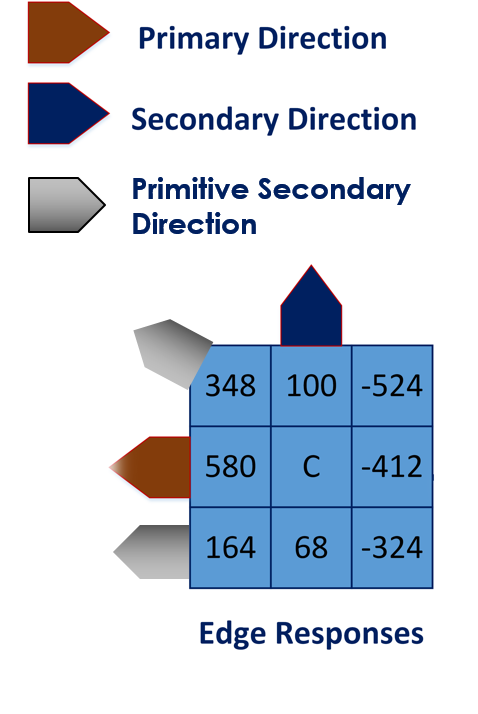
\includegraphics[width=0.4\textwidth]{primary_secondary_ER.png}
		\caption{Primary and Secondary Edge Response Selection}
				\label{fig:primary_secondary_ER}
	\end{center}
\end{figure}


\subsubsection{Step 3: Threshold($\sigma$) generation} 
We need a threshold to generate magnitude code as in equation . We introduce a global adaptive thresholding schema to differentiate the flat region from high-textured region.We carefully observe the characteristics of flat textures in a face image and found that, for a flat patch, edge responses are low and close to each other. It is also evident that, flat textures are dominant among all texture patterns in a face image and mostly appear in the cheek region. To generate threshold ($\sigma$), we take the median of the primary edge responses in the cheek region. 

To find the cheek region as shown in figure \ref{fig:Cheek_Region}, we use Active Appearance Model (AAM) that provides us 68 landmarks for each image and we select following four landmarks among them.
\begin{itemize}
	\item most left eyebrow point
	\item most right eyebrow point
	\item most lower eye point
	\item most upper lip point\\
	These four landmarks form a rectangle that defines the cheek region.	
\end{itemize}  
\begin{figure}[H]
	\begin{center}
		\centering
		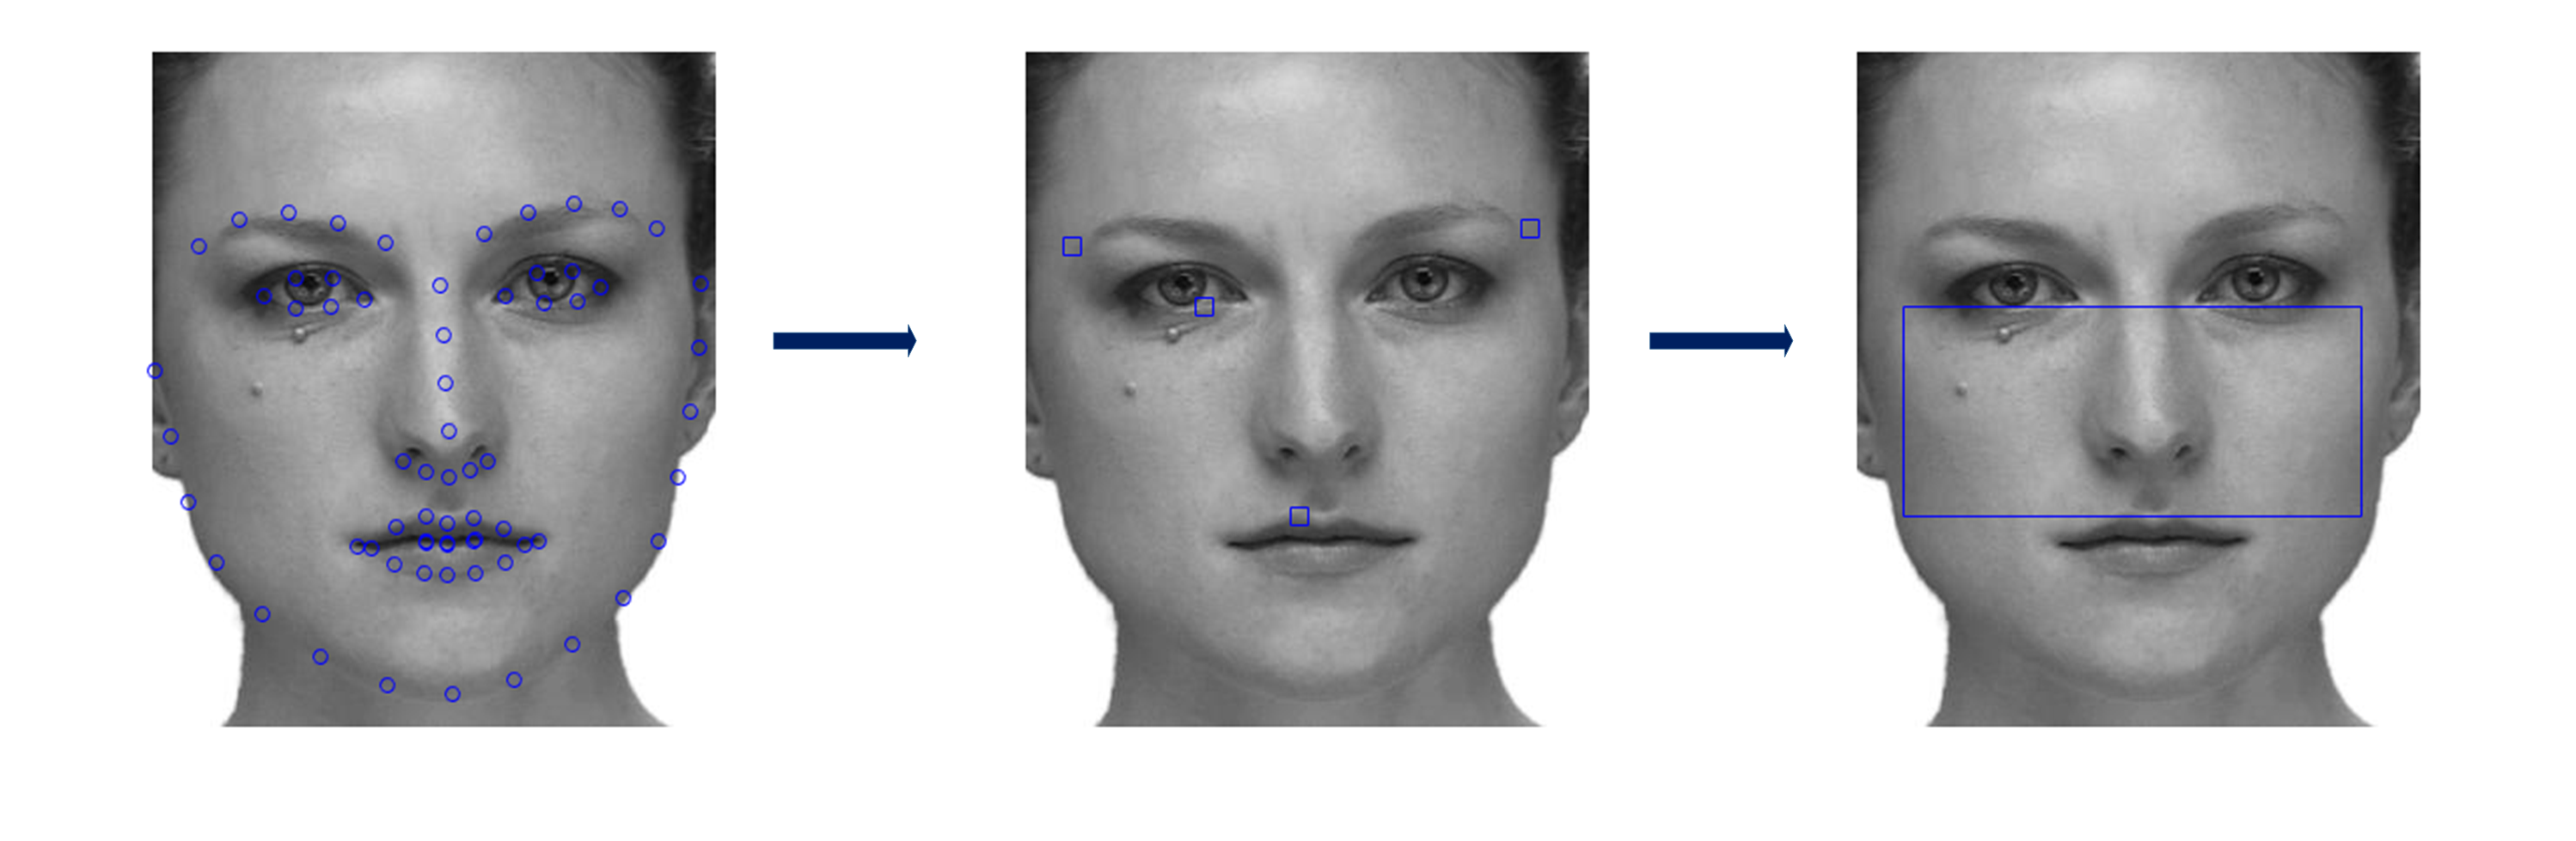
\includegraphics[width=\textwidth]{Cheek_Region.png}
		\caption{Cheek Region}
			\label{fig:Cheek_Region}
	\end{center}
\end{figure} 

\subsubsection{Step 4: Sign, Magnitude, Direction and Center codes generation} 
Given a pixel, ARLCP Sign (ARLCP\_S) is generated based on the information of sign of edge responses as:
\begin{equation}
ARLCP\_S=\sum\limits_{i=0}^{p-1}{s({{E}_{i}}){{2}^{i}}}; \tab  s(x)= 
\begin{cases}
1,& \text{if } x\geq 1\\
0,& \text{otherwise}
\end{cases}
\label{equation:ARLCPss}
\end{equation}

Here, E$_i$ refers to i$^{th}$ edge response. If the edge response is positive, it is set to 1 and 0 otherwise. Then the binary pattern is encoded to decimal shown in figure \ref{fig:sign} that represents the sign code of the pixel.
\begin{figure}[H]
	\begin{center}
		\centering
		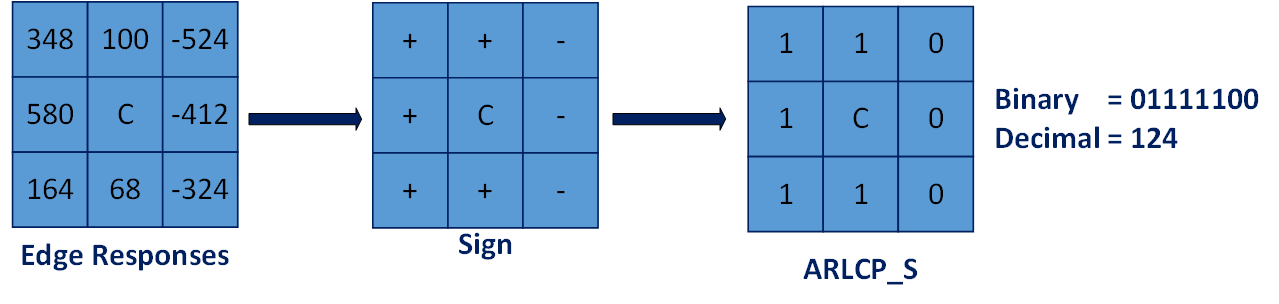
\includegraphics[width=\textwidth]{sign.png}
		\caption{ARLCP\_S generation}
		\label{fig:sign}
	\end{center}
\end{figure}

To get the information how significant the edge response in each direction, ARLCP Magnitude (ARLCP\_M) code is generated that can be defined as: \\


\begin{equation}
ARLCP\_M=\sum\limits_{i=0}^{p-1}{s(|{{E}_{i}}|-\sigma ){{2}^{i}}}
\label{eqn:arlcpM}
\end{equation}
Here, $\sigma$ is the adaptive threshold generated in step 3. Edge response with higher magnitude with respect to $\sigma$ is considered as 1 and 0 otherwise. Figure \ref{fig:mag} illustrates ARLCP Magnitude (ARLCP$_M$) code generation. Here, threshold $\sigma$ has value of 196.
\begin{figure}[H]
	\begin{center}
		\centering
		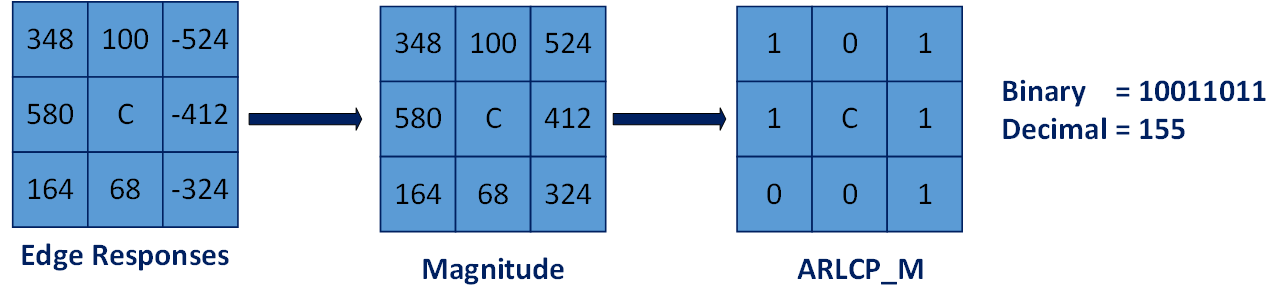
\includegraphics[width=\textwidth]{mag.png}
		\caption{ARLCP\_M generation}
		\label{fig:mag}
	\end{center}
\end{figure}

Along with the sign and magnitude of edge response, we also incorporate direction information. Figure \ref{fig:dir}(a) shows all the eight directions we have considered. Primary and secondary edge direction selected in step 2 are concatenated as equation (\ref{equation:dir}) and generate ARLCP Direction (ARLCP\_D) code as shown in figure \ref{fig:dir}(b) that represents the Direction code of the pixel.\\
\begin{equation}
 ARLCP\_D = [d_1 ,d_2]
 \label{equation:dir}
\end{equation}
\vspace*{0.5cm}
\begin{figure}[H]
	\begin{center}
		\centering
		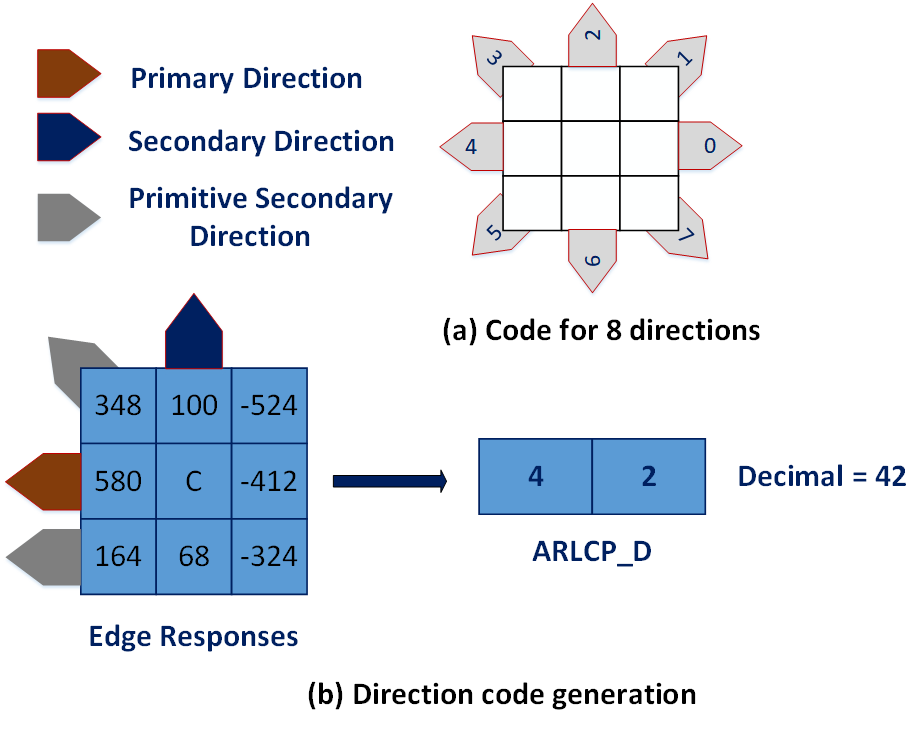
\includegraphics[width=0.7\textwidth]{dir.png}
		\caption{ARLCP$_D$ generation}
		\label{fig:dir}
	\end{center}
\end{figure}

Finally ARLCP Center (ARLCP\_C) code is generated thresholding the given pixel with respect to average intensity value of entire image, ($\gamma$) shown in figure \ref{fig:center}. Here, threshold $\gamma$ has value of 64. ARLCP\_C can be defied as:\\

\begin{equation}
 ARLCP\_C = S(g_c-\gamma)
 \label{equation:center}
\end{equation}
\vspace*{0.5cm}
\begin{figure}[H]
	\begin{center}
		\centering
		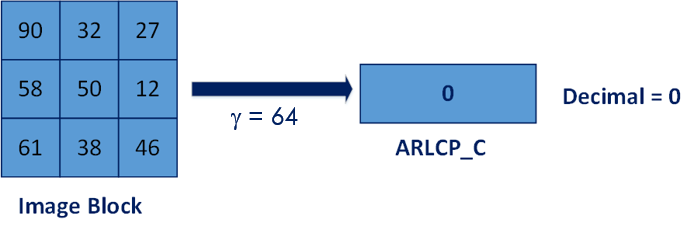
\includegraphics[width=0.7\textwidth]{center.png}
		\caption{ARLCP\_C generation}
		\label{fig:center}
	\end{center}
\end{figure}


In essence, Figure \ref{fig:Code_generation} illustrates how all these four codes are generated from an 3x3 image block. The initial value in the block is the intensity of the 9 pixels in the block. Likewise each pixel of the image generates 8 directional responses. Edge response magnitudes are more stable than intensity values in presence of noise and illumination variation and the use of edge response in our method makes it more robust in presence of noise and lighting variation. After calculating the edge responses, we select top two edge responses defined as primary and primitive secondary edge response respectively. And we select secondary edge response avoiding neighbors of primary edge response. Then Sign and magnitude of edge responses are generated. Here ARLCP Sign (ARLCP\_S) code is generated by converting negative values to zeros and positive values to ones. In case of  ARLCP Magnitude (ARLCP\_M) code generation, magnitudes greater or equal to threshold $\sigma$ are considered as 1 and 0 otherwise. Here, $\sigma$ is calculated from the median primary edge response in the cheek region. After that, we concatenate the directions of primary and secondary edge responses to get ARLCP Direction (ARLCP\_D) code. Lastly we generate ARLCP Center (ARLCP\_C) code by thresholding center pixel in a block of 3x3 neighborhood.
\vspace*{0.5cm}
\begin{figure}[H]
	\begin{center}
		\centering
		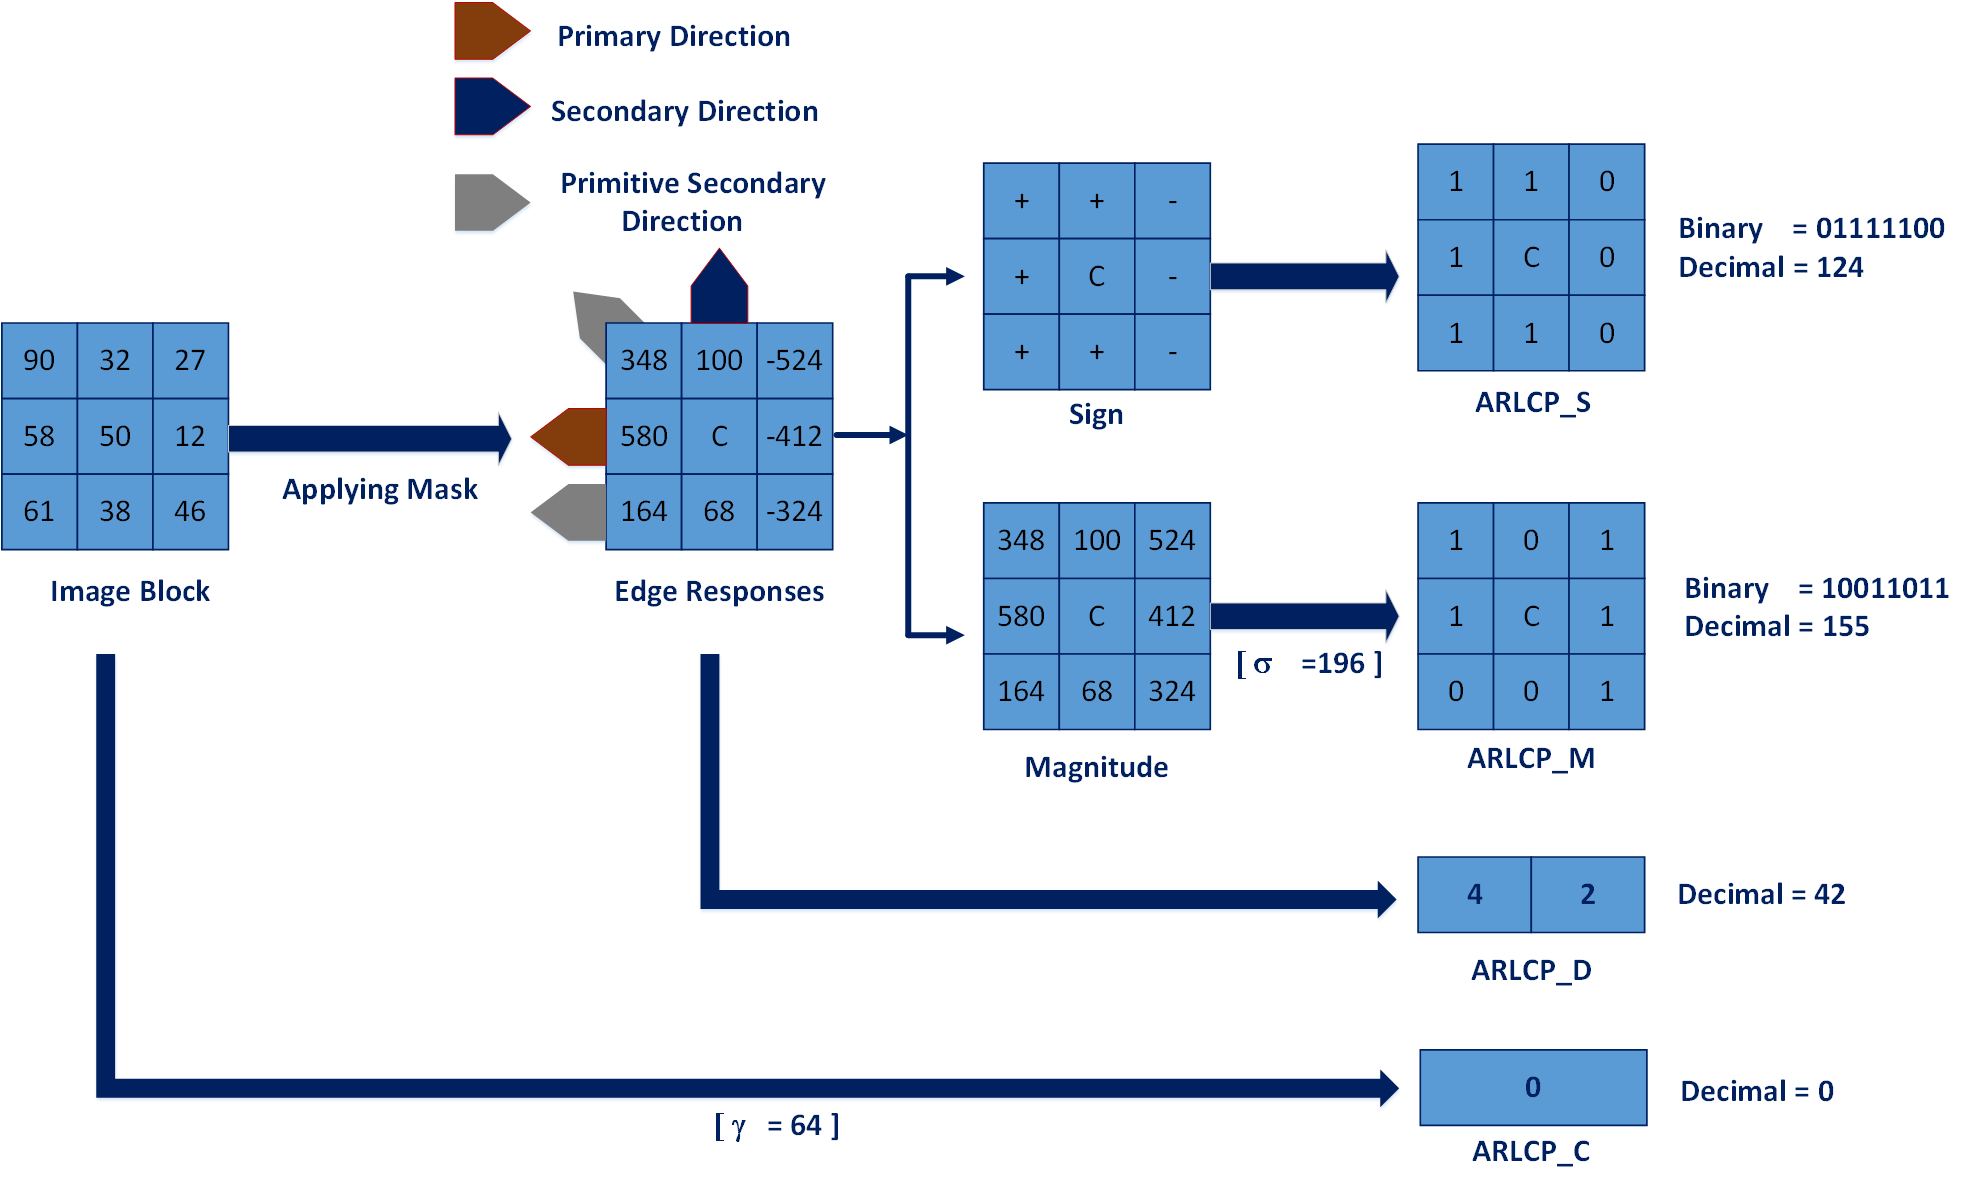
\includegraphics[width=\textwidth]{Code_generation.png}
		\caption{ARLCP codes generation}
		\label{fig:Code_generation}
	\end{center}
\end{figure}


\subsubsection{Step 5: Histograms of Sign, Magnitude, Direction and Center codes generation} 
Histogram is generated for each of the ARLCP\_S, ARLCP\_M, ARLCP\_D, ARLCP\_C code following the equation \ref{histo1}, \ref{histo2} and concatenated to generate the final feature vector that represents an image. Figure \ref{fig:histogram_generation} depicts the final feature generation. Here $H^k$ represents histogram of $k^{th}$ region.


\begin{equation}
{{H}^{k}}(c)~=\sum\limits_{(x,y)\in {{R}^{k}}}{\partial (P(x,y)),c),}~\forall c
\label{histo1}
\end{equation}

\begin{equation}
\partial ~(a,b)=\left\{ \begin{matrix}
1 ~~~ a=b  \\
0 ~~~ a\ne b  \\
\end{matrix} \right.
\label{histo2}
\end{equation}
\vspace*{0.5cm}
\begin{figure}[H]
	\centering
	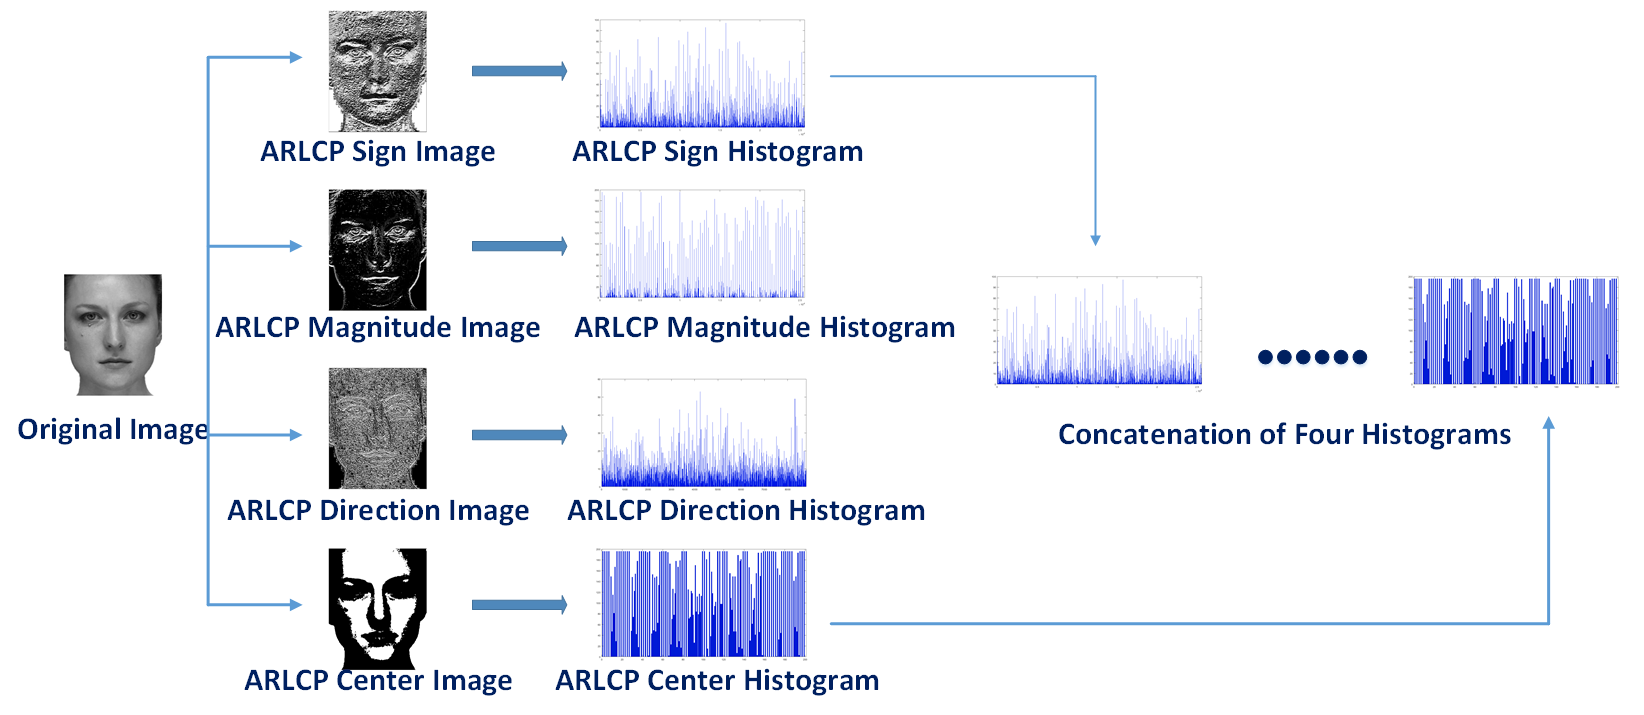
\includegraphics[width=0.9\textwidth]{histogram_generation.png}
	\caption{Histogram Generation}
	\label{fig:histogram_generation}	
\end{figure}	

\subsection{Facial Feature Representation with ARLCP}
To retain more spatial information, an image is divided into $n\times n$ regions (e.g. $10 \times 10$, $5 \times 5$).
Applying the ARLCP operator on all the pixels of a region will result in four ARLCP histograms as ARLCP\_S, ARLCP\_M, ARLCP\_D and ARLCP\_C. Then these four histograms are concatenated to form a feature vector of that region. Finally feature vectors for all regions are concatenated to generate final feature vector as shown in figure \ref{fig:Local_histogram} that represents the image.
\vspace*{0.5cm}
\begin{figure}[H]
	\begin{center}
		\centering
		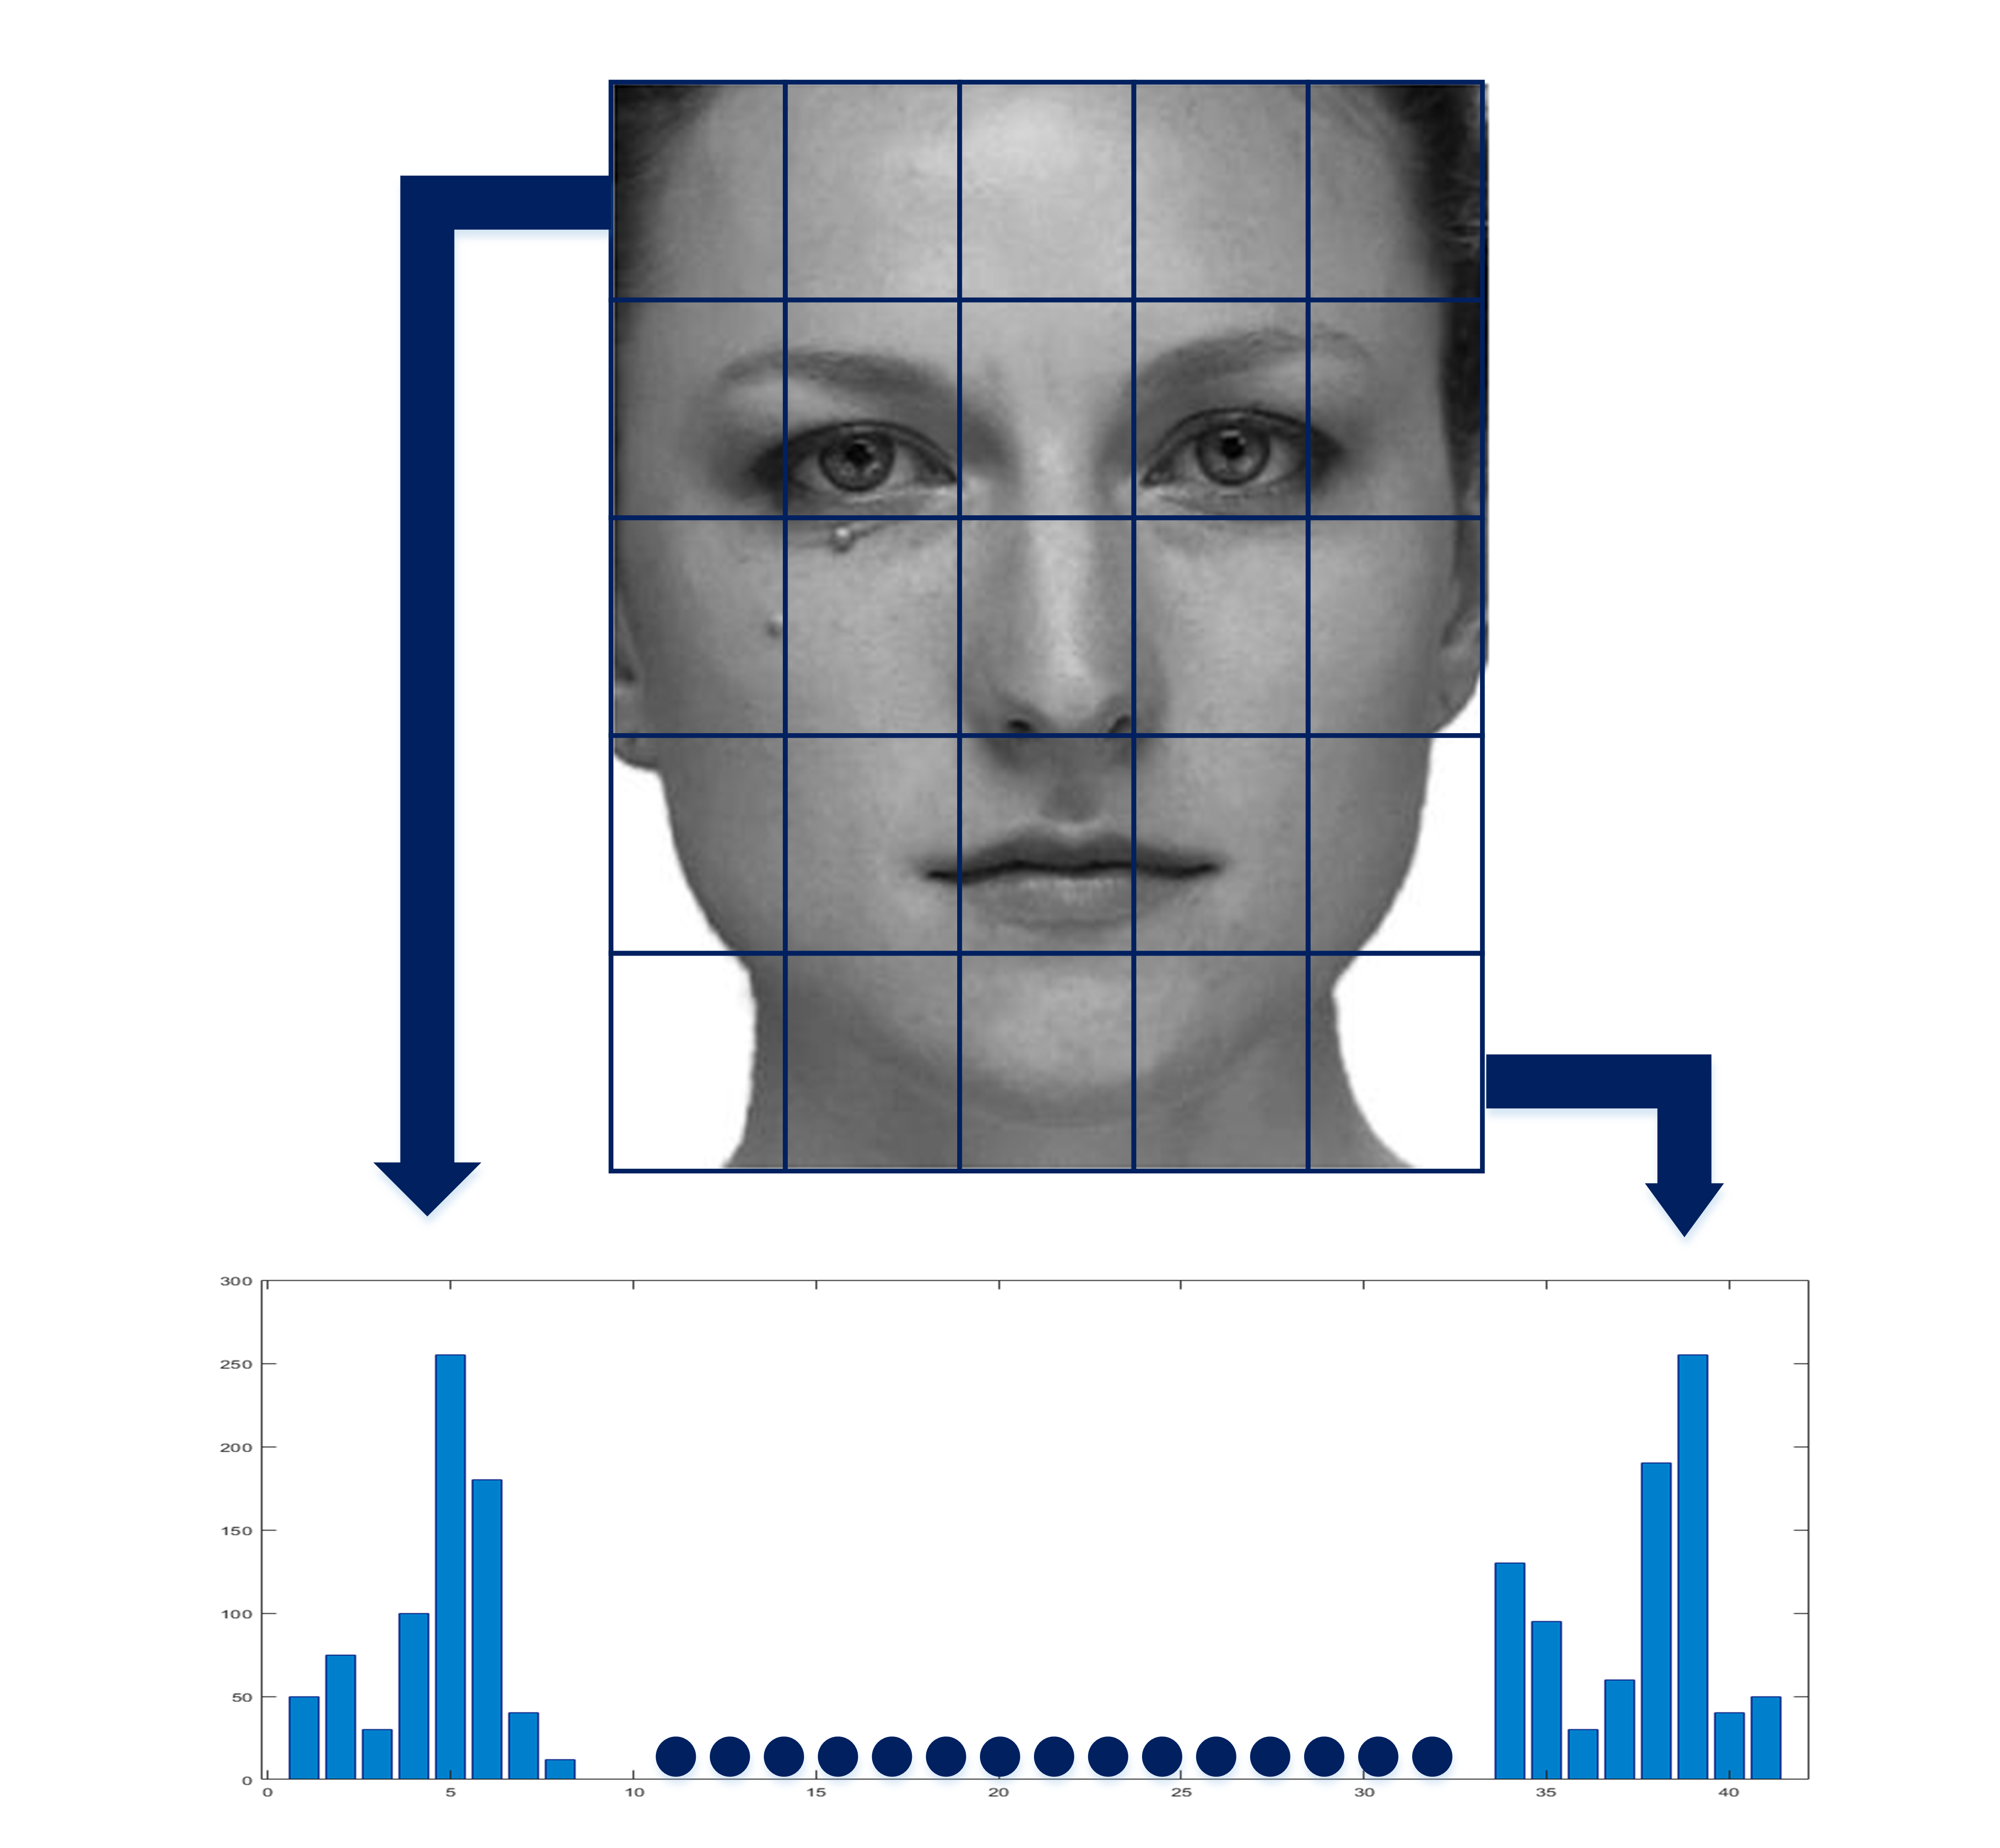
\includegraphics[width=0.5\textwidth]{Local_histogram.png}
		\caption{Local Histograms Concatenation}
		\label{fig:Local_histogram}
	\end{center}
\end{figure}

\subsection{Expression Recognition using KNN Classifier}
We experiment our proposed feature descriptor Adaptive Robust Local Complete Pattern (ARLCP) with K-Nearest Neighbor (KNN) to recognize different facial expressions. We take images and generate feature vector for each image using ARLCP and then use the feature vectors as input to KNN for classifying the class of the images.

The KNN algorithm is a robust and versatile classifier that falls in the supervised learning family of algorithms. Informally, this means that we are given a labelled dataset consiting of training observations (x,y) and would like to capture the relationship between x and y. More formally, our goal is to learn a function \textit{h:X$\rightarrow$Y} so that given an unseen observation \textit{\textbf{x, h(x)}} can confidently predict the corresponding output y.

When KNN is used for classification, the output can be calculated as the class with the highest frequency from the K-most similar instances. Each instance in essence votes for their class and the class with the most votes is taken as the prediction. Similarity is defined according to a distance metric between two data points. A popular choice is the Euclidean distance given by
\begin{equation}
d(x,x')=\sqrt{(x_1-x'_1)^2+(x_2-x'_2)^2+...+(x_n-x'_n)^2}
\end{equation}

\noindent Also there are other measures like Manhattan, Chebyshev and Hamming distance. More formally, given a positive integer K, an unseen observation x and a similarity metric d, KNN classifier performs the following two steps:
\begin{itemize}
	\item KNN runs through the whole dataset computing d between x and each training observation. Lets say, A be the set of k points in the training data that are closest to x. K is usually odd to prevent tie situations.
	\item  Then the conditional probability for each class is estimated, that is, the fraction of points in A with that given class label as:
	
	\begin{equation}
	P(y=j,X=x)=\frac{1}{K}\sum_{i\epsilon A}^{}I(y^i=j)
	\end{equation}
\end{itemize}	
\noindent Here, I(x) is the indicator function which evaluates to 1 when the argument x is true and 0 otherwise. The class with highest probability is assigned to the given sample.
\begin{figure}[H]
	\begin{center}
		\centering
		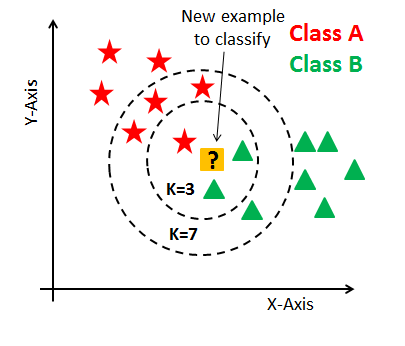
\includegraphics[width=0.8\textwidth]{KNN.png}
		\caption{KNN Classification}
		\label{fig:KNN_Classification}
	\end{center}
\end{figure}
\noindent Figure \ref{fig:KNN_Classification} illustrates how KNN classifier classifies a given sample with 2 dimensional feature for different values of K. \noindent Here, KNN classifies a given sample to class B when K=3 as within the three closest training samples, two samples are from class B. But in case of K=7, four out of seven training samples are from class A. So KNN classifies the given sample as class A. Therefore, classification can be different for different value of K.


\subsection{Strengths of the Proposed Descriptor}
Here we discuss the good properties of our proposed face descriptor for facial expression
recognition. Some strengths of the proposed feature descriptor are:
\begin{itemize}
	\item Instead of direct pixel, this method uses directional edge response that is more robust to noise and illumination variation.
	\item This method uses directional information along with sign and magnitude of edge responses that leads to more unique representation of an image.
	\item Instead of static threshold for all image, this method uses an adaptive threshold for each image as static threshold on primary response is quite sensitive since it may wipe-out either edge pixels in low-contrast image or flat pixels in natural noisy images
	\end {itemize}
	
	
	

\newpage
\section{Experimental Result}
\subsection{Experimental Setup and Dataset Description}
The JAFFE database \cite{lyons1998coding} comprises facial expression images of 10 Japanese female subjects. All the images were digitized into a resolution of 256x256 pixels. The
images were taken from a frontal pose, and the subjects' hair was tied back in
order to facilitate the exposure of all the expressive zones of the face. In the
image scene, an even illumination was created using tungsten lights. Instead of
revealing the actual names, the subjects are referred with their initials, which are KA, KL, KM, KR, MK, NA, NM, TM, UY, and YM. In our setup,the expression dataset comprises a total of 213 images.\\

\begin{figure}[h]	
	\centering
	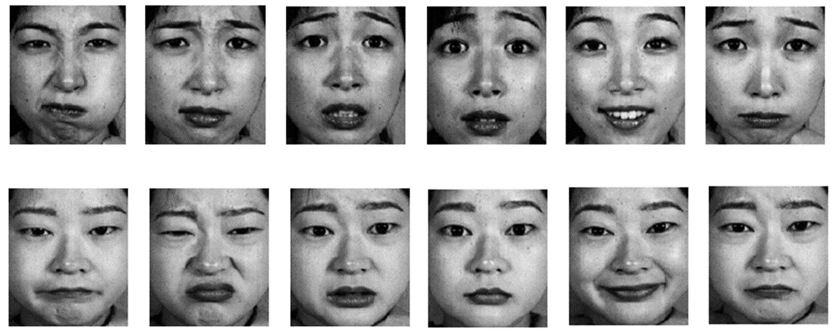
\includegraphics[width=0.5\textwidth]{jaffe}
	\caption{JAFFE Database}		
\end{figure}

The Extended Cohn-Kanade Facial Expression (CK+) database \cite{lucey2010extended} comprises 593 image sequences (from neutral	to apex) of 123 subjects who were instructed to perform a series of 23 facial displays. From these sequences, 327 out of 593 have each of the seven basic emotion categories: anger, contempt, disgust, fear, happiness, sadness and surprise. In our setup, we selected 327 sequences with 7 emotion categories.The three most expressive image frames were selected from each sequence to make the 7-class expression dataset (981 images).
\begin{figure}[h]
	\centering
	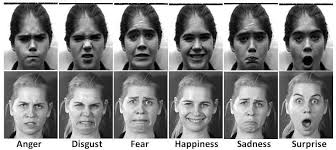
\includegraphics[width=0.5\textwidth]{images_ck+}
	\caption{CK+ Database}		
\end{figure}

Ryerson Audio-Visual Database of Emotional Speech and Song (RAVDESS) We use 4904 videos from RAVDESS dataset \cite{livingstone2018ryerson}. We collect 50 frames from each videos that leads to total 245,200 images with 8 emotion categories ( neutral, calm, happy, sad, angry, fearful, disgust, surprised ). The selected images were cropped from the original and then normalized to 320x380 pixels.
\begin{figure}[h]	
	\centering
	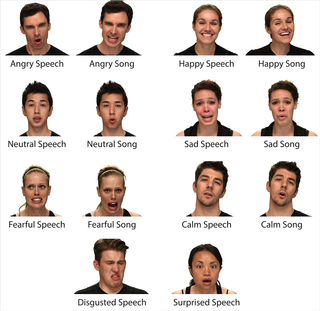
\includegraphics[width=0.5\textwidth]{images_ravdess}
	\caption{Ravdess Database}		
\end{figure}

\subsection{Performance Evaluation}
In order to evaluate the proposed method in expression recognition, we carried out
a five-fold cross-validation to measure the classification rate. In a five-fold cross-validation, the whole dataset is randomly partitioned into five subsets, where
each subset comprises an equal number of instances. One subset is used as the testing set and the classifier is trained on the remaining nine subsets. The average classification rate is calculated after repeating the above process for five times. K-Nearest Neighbor is used as the classifier. We present the performance of the experiments with accuracy which is defined as:
$$\text{Accuracy}=\frac{\text{Number of correctly classified samples}}{\text{Total number of test samples}}$$
\subsection{Performance on JAFFE Database}
For the JAFFE database, we have compared the performance of the proposed method with other well-known local pattern operators, namely local binary pattern (LBP) \cite{shan2005robust}, local ternary pattern (LTP) \cite{tan2010enhanced}, local directional pattern (LDP) \cite{jabid2010robust}, Complete Local Binary Pattern(CLBP)\cite{clbp01} and Adaptive Robust Binary Pattern(\cite{arbp01}) . We used K Nearest Neighbor (KNN) to classify the test samples and measure the accuracy by counting  the correctly classified samples. We used five-fold cross validation scheme to evaluate the performance.

\begin{table}[H]
	\begin{center}
		\caption{Recognition rate (\%) for the JAFFE 7-class expression dataset.}
		\begin{tabular}{|c|c|}
			
			\hline
			\textbf{Feature Descriptor } & \textbf{Accuracy (\%)}\\
			\hline
			LBP & 88.21 \\
			LTP & 88.67 \\
			LDP & 89.52 \\
			CLBP & 88.83 \\
			ARBP & 92.51 \\
			ARLCP & 94.41 \\
			\hline
			
		\end{tabular}
		 
		\label{tab:jaffe_recognition_rate}
	\end{center}
\end{table}


\noindent Table \ref{tab:jaffe_recognition_rate} shows the recognition rate of our proposed ARCLP along with local pattern-based feature descriptors LBP, LTP, LDP, CLBP and ARBP against the 7-class expression JAFFE dataset. It can be observed that, ARLCP exhibits superior performance in recognizing expression images. However, JAFFE dataset contains fewer images than CK+ dataset. So we cannot ensure sufficient sample image for training and some expressions are labeled incorrectly or expressed wrongly. Therefore, the results from JAFFE dataset should be lower than CK+ dataset.

\subsection{Performance on CK+ Database}
For the CK+ database, the ARLCP feature descriptor achieves classification rate
of 98.67\%. Table \ref{tab:ck_plus_recognition_rate} shows the recognition rates of different feature
descriptors with the CK+ 7-class expression dataset. It can be observed that, ARLCP achieves the highest classification rate.

\begin{table}[H]
	\begin{center}
		\caption{Recognition rate (\%) for the CK+ 7-class expression dataset.} 
		\label{tab:ck_plus_recognition_rate}
		
		\begin{tabular}{|c|c|}
			
			\hline
			\textbf{Feature Descriptor } & \textbf{Accuracy (\%)}\\
			\hline
			LBP & 90.21 \\
			LTP & 95.67 \\
			LDP & 95.73 \\
			CLBP & 96.94 \\
			ARBP & 97.56 \\
			ARLCP & 98.67 \\
			\hline
			
		\end{tabular}
	\end{center}
\end{table}
\noindent We generate confusion matrix for CK+ dataset using ARLCP feature descriptor shown in table \ref{tab:ck_plus_confusion_matrix} where diagonal values define the matching with the original data and non-diagonal values show the mismatch.\\
\begin{table}[H]
	\begin{center}
				\caption{Confusion matrix for the CK+ 7 dataset -class recognition using ARLCP feature representation.} 
		\begin{tabular}{|c|c|c|c|c|c|c|c|c|}
			
			\hline
			& & 1 & 2 & 3 & 4 & 5 & 6 & 7 \\
			\hline
			1 & Anger & \textbf{96.4} & 0 &  3.6 & 0 & 0 &  0  & 0 \\
			\hline
			2 & Contempt & 0 & \textbf{100} & 0 & 0 & 0 &  0  & 0  \\
			\hline
			3 & Disgust & 0  & 0 & \textbf{97.34} & 0 & 2.66 &  0  & 0  \\
			\hline
			4 & Fear & 0  & 0  & 0 & \textbf{100} & 0 &  0  & 0  \\
			\hline
			5 & Happy & 0 & 0 & 0 & 0 & \textbf{100} & 0 & 0  \\
			\hline
			6 & Sadness & 0 & 0 & 3.05 & 0 &  0 & \textbf{96.95} & 0  \\
			\hline
			7 & Surprise & 0 & 0 & 0 & 0 &  0  & 0 & \textbf{100}  \\
			\hline
			
			
		\end{tabular}
		\label{tab:ck_plus_confusion_matrix}
		
	\end{center}
\end{table}

Here we can see here, the expression ``Anger'' has 96.4\% accuracy and 3.6\% of it mismatches with the disgust expressions as they are very close. Similarly, 2.66\% of ``Disgust'' expressions have been matched with the ``Happy'' faces. Also, ``Sadness'' conflicted with the ``Disgust'' faces at 3.05\%.\\

To investigate the robustness of the proposed ARLCP descriptor under the presence
of noise, further experiments are conducted on the images from the CK+ 7-class expression dataset. In the experimental setup, the images are contaminated with Gaussian noise of different variances. Figure \ref{fig:CK_plus_noisy} shows the recognition rate for images corrupted with noise of mean 0 and different variances (0.02, 0.03 and 0.04), experimented with different operators. We have observed that ARLCP provides better accuracy than other existing local operators.

\begin{figure}[H]
	\begin{center}
		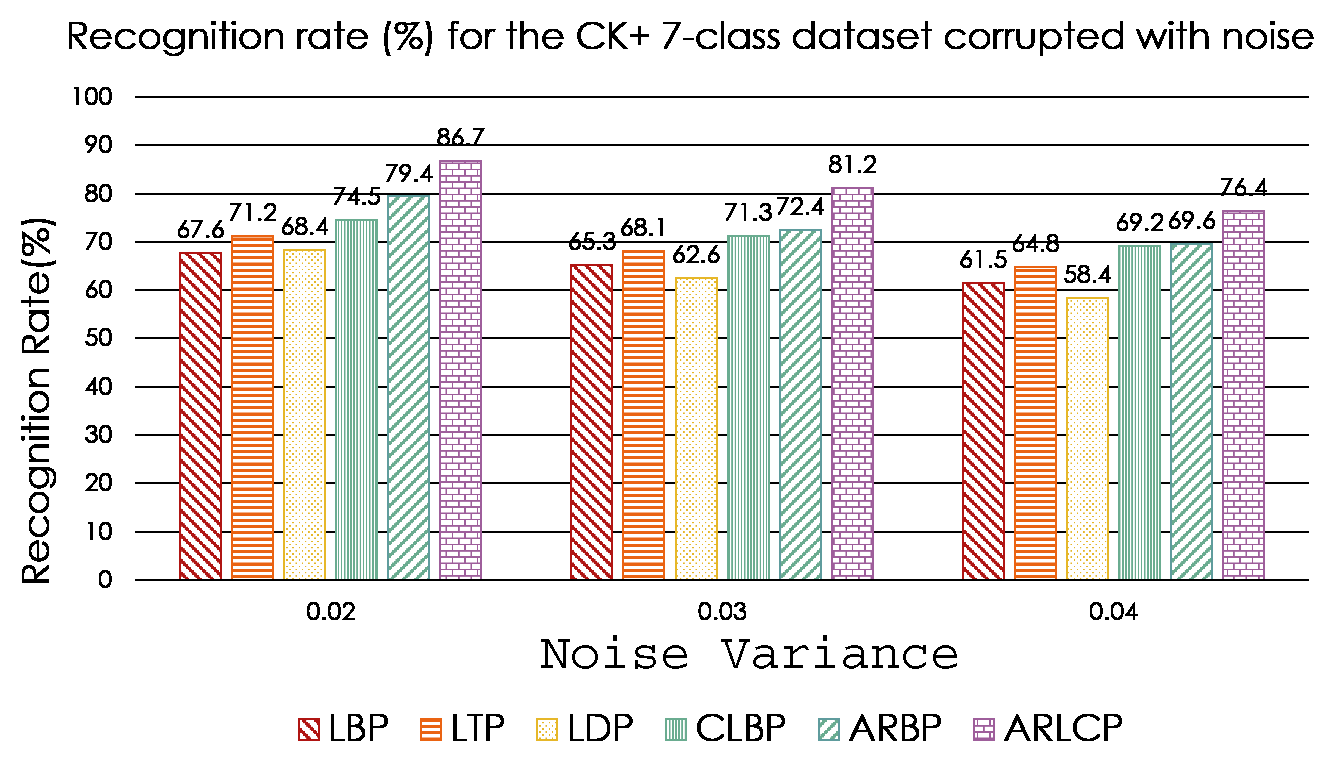
\includegraphics[width=\textwidth]{Picture4.png}			
		\caption{Recognition rate (\%) for the CK+ 7-class dataset corrupted with noise}
		\label{fig:CK_plus_noisy}
	\end{center}
\end{figure}


Our proposed method ARLCP also shows better performance in case of lower resolution. Automated facial analysis is useful in smart meeting, surveillance and many other
applications, where often only low-resolution video data is available. Since geometric
methods like detection of facial action units are difficult to accommodate in these scenarios, appearance-based methods seem to be a better solution. Therefore, the performance of the proposed method is also evaluated on low-resolution images. We experiment with different resolution and observe that our method exhibits superior performance. Figure \ref{fig:ck_plus_resolution} shows the recognition rate for CK+ dataset with different resolution.

\begin{figure}[H]
	\begin{center}
		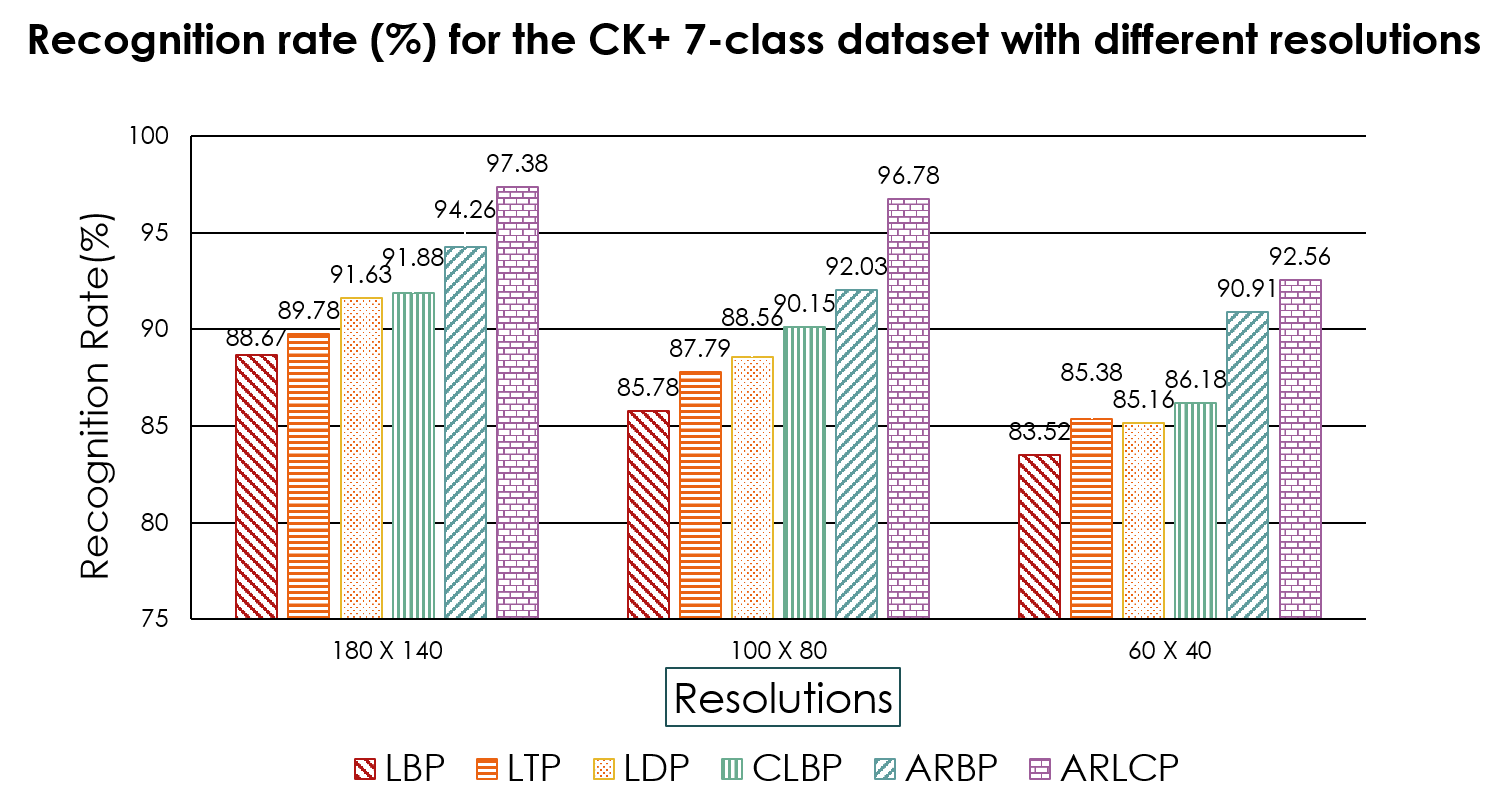
\includegraphics[width=\textwidth]{Picture5.png}			
		\caption{Recognition rate (\%) for the CK+ 7-class dataset with different resolutions}
		\label{fig:ck_plus_resolution}
	\end{center}
\end{figure}

It is important to retain spatial information as much as possible and it can be achieved by dividing the images into more number of regions. Hence, we also experimented our proposed method dividing the images with different number of regions such as $10 \times 10$, $5 \times 5$ and $2 \times 2$. However, excessively increasing the number of regions may result in the decrease of accuracy as there will be less number of pixels in each region. Here we compare ARLCP with other methods and it can be observed that ARLCP provides better accuracy. Figure \ref{fig:ck_plus_region} shows the recognition rate for  CK+ dataset divided by several number of regions.

\begin{figure}[H]
	\begin{center}
		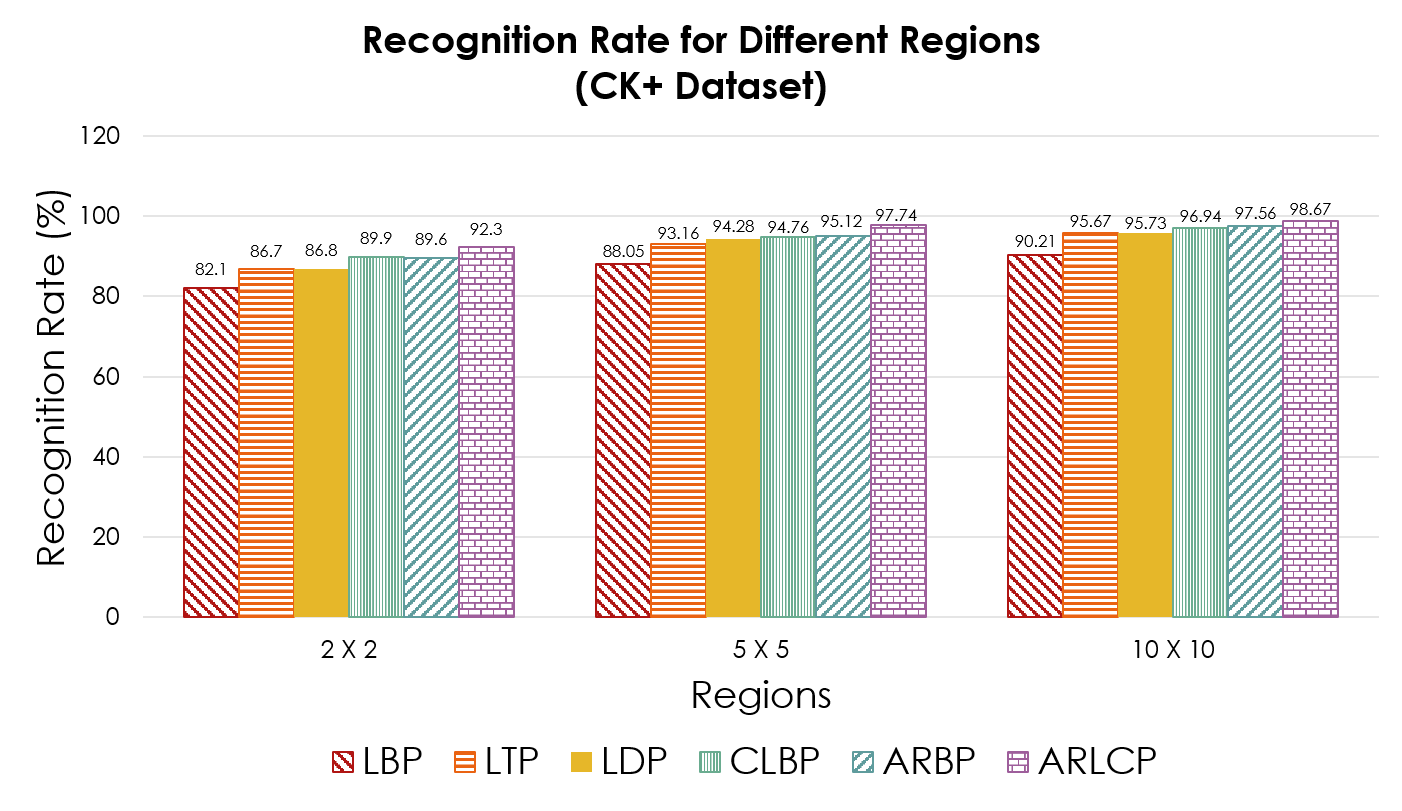
\includegraphics[width=\textwidth]{a.png}			
		\caption{Recognition Rate(\%) for Different Regions (CK+ Dataset)}
		\label{fig:ck_plus_region}
	\end{center}
\end{figure}

\subsection{Performance on RAVDESS Database}
For the RAVDESS dataset, ARLCP achieves Recognition rate of 99.90\% and 99.86\% using KNN classifier with 10-Fold and 5-fold cross validation respectively. Table \ref{tab:RAVDESS_confusion_matrix} shows the confusion matrix for RAVDESS dataset with 5-fold cross validation.

\begin{table}[H]
	\begin{center}
			\caption{Confusion matrix for the RAVDESS 8-class recognition using	ARLCP feature representation with 10-fold cross validation} 
		\begin{tabular}{|c|c|c|c|c|c|c|c|c|c|}
			
			\hline
			& & 1 & 2 & 3 & 4 & 5 & 6 & 7 & 8 \\
			\hline
			1 & Neutral & \textbf{99.8} & 0.13 &  0 & 0 & 0.07 &  0  & 0 & 0 \\
			\hline
			2 & Calm & 0.08 & \textbf{99.8} & 0.03 & 0 & 0.03 &  0  & 0.03 & 0.03  \\
			\hline
			3 & Happy & 0  & 0 & \textbf{100} & 0 & 0 &  0  & 0 & 0  \\
			\hline
			4 & Sad & 0  & 0  & 0 & \textbf{99.9} & 0 &  0.1  & 0 & 0  \\
			\hline
			5 & Angry & 0 & 0 & 0 & 0 & \textbf{99.9} & 0.05 & 0.05 & 0  \\
			\hline
			6 & Fearful & 0.03 & 0 & 0.03 & 0 &  0.14 & \textbf{99.8} & 0.03 & 0  \\
			\hline
			7 & Disgust & 0 & 0 & 0 & 0.05 &  0.05  & 0 & \textbf{99.9} & 0  \\
			\hline
			8 & Surprised & 0 & 0 & 0 & 0 & 0 &  0  & 0 & \textbf{100} \\
			\hline
			
			
		\end{tabular}
	
		\label{tab:RAVDESS_confusion_matrix}
	\end{center}
\end{table}


\newpage

\section{Conclusion}
\label{chap:ch3}

\subsection{Research Summary}
The thesis aims to design a robust facial feature representation that overcomes the limitations of existing approaches and can be used in facial expression recognition. 

In this thesis we introduced a new local texture pattern, the Adaptive Robust Local Complete Pattern (ARLCP). The descriptor uses sign, magnitude and directional information of edge responses.Therefore, this operator is more robust to noise and illumination variation. The ARLCP operator also integrates adaptive threshold instead of a static one as static threshold on primary edge response is quite sensitive to noisy and low-contrast images. The proposed method has been evaluated for facial expression recognition classification. Experiments using different benchmark datasets exhibits better performance of ARLCP against other well-known appearance-based feature descriptors namely LBP, LTP, LDP, CLBP, ARLBP. As four histograms are concatenated to generate final feature vector, execution time increases. 

The ARLCP operator provides robustness to noise and illumination variation, higher discriminating capability compared to existing feature descriptors. Therefore, it can be effectively used in facial expressions recognition. 

\newpage	
\subsection{Future Works }				

In our proposed method, we considered static images for facial expression recognition. In future, we plan to use our method for facial expression recognition from video sequence images. Also we plan to optimize the method to reduce the feature dimension as well as time complexity.
\newpage
\addcontentsline{toc}{section}{References}
\bibliography{thesisbiblio}
\bibliographystyle{IEEEtran}
\end{document}